\documentclass[11pt,a4paper]{article}
\usepackage[all]{xy}
\usepackage{amsmath, amssymb}
\usepackage{algorithm, algorithmicx, algpseudocode}
\usepackage{stmaryrd}
\usepackage{color}
\usepackage{graphicx}
\usepackage[utf8]{inputenc}
\usepackage{hyperref}
\usepackage{url} %Shouldn't be needed
\usepackage{tikz}
\usepackage{booktabs}
\usepackage[toc]{appendix}
\usetikzlibrary{arrows, automata, positioning}
%\usepackage[natbibapa]{apacite}

%Settings
\hypersetup{
	colorlinks=false,
	bookmarks=true,
	linkcolor=blue
}
\graphicspath{{./Pics/}}
\numberwithin{figure}{section}
\bibliographystyle{plain}

%\usepackage[rightcaption]{sidecap}
%\usepackage{float}

%Commands
\newcommand{\todo}[1]{\textcolor{cyan}{(TODO: #1)}}
\newcommand{\question}[1]{\textcolor{red}{(ASK TRULS: #1)}}
\newcommand{\bisim}{\mathfrak{R}}

%Commonly used variables
\newcommand{\states}{S}
\newcommand{\rels}{\sim}
\newcommand{\ags}{A}
\newcommand{\vals}{V}
\newcommand{\props}{P}
\newcommand{\model}[1]{$M#1 = (\states#1, \rels#1, \vals#1)$}
\newcommand{\lang}[1]{$\mathcal{L}_{#1}$}
\newcommand{\M}{\mathcal{M}}
\newcommand{\dia}[1]{\langle#1\rangle}
\newcommand{\eqc}[1]{\llbracket#1\rrbracket}
\newcommand{\ext}[1]{||#1||}
\newcommand{\labels}[1]{F_{#1}}
\newcommand{\anns}[1]{\mathcal{A}_{#1}}
\newcommand{\cname}{GALMC}

%Enviroments
\newtheorem{thm}{Theorem}[section]
\newtheorem{cor}[thm]{Corollary}
\newtheorem{lem}[thm]{Lemma}
\newtheorem{conjecture}[thm]{Conjecture}
\newtheorem{definition}[thm]{Definition} %Make definitions start on new line?
\newtheorem{proposition}[thm]{Proposition}
\newtheorem{example}[thm]{Example}
\newtheorem{fig}{Figure}[section]

\begin{document}

\author{Anders Eide}
\title{To be announced: \\\large Understanding and model checking Group Announcement Logic}
\date{Sometime in the future}

\maketitle
\question{Hvordan pynte dette?}

\newpage
\tableofcontents

%Insert UiB Owl at some point \newpage
\section*{Abstract}

In this master's thesis we present a graphical model checking tool for group announcement logic called \cname, capable of visualizing the process of checking formulas in a step-by-step fashion. We also define how to enumerate the set of ways a given coalition can restrict a model as well as present pseudocode algorithms describing how we translated these definitions in our model checker. 

 \newpage
\section{Introduction}\label{sec:intro}

\subsection{Motivation}

\question{Greit med førsteperson i motivasjon?}\\
\todo{Skriv om hele introduksjonen av GAL}\\
\todo{Hente ned bilder av JFLAP i aksjon, med illustrasjoner av hvordan verktøyet og stepperen i det fungerer}\\

%Research questions

%Can we create a model checking tool for GAL
%That can enumerate the set of announceable extensions for a given coalition
%And also visually present the process of checking formulas


%JFLAP: 
%Started as a set of tools at Rensselaer Polytechnic Institute around 1990, moved to Duke University in 1994
%The creators of JFLAP describe it as "a package of graphical tools which can be used as an aid in learning the basic concepts of Formal Languages and Automata Theory."
%JFLAP introduces the concept of turing machines which can be rather abstract for a fledgeling student to grasp


%Symbolic Model Checking
%SMCDEL, symbolic model checker for dynamic epistemic logic including a variant of group announcements
%

\todo{Write sub-section on inspiration for tool about JFLAP, educational benefits ect}

%While measuring the educational benefit of our tool is beyond the scope of this thesis, we at least hope to put a tool out there so that others can use it in their courses and potentially leading to more papers on the topic in the future.
\question{Footnotes i en masteroppgave? Lenke til nettsiden for JFLAP}

In 2010, Ågotnes et al. submitted a paper on their extension of Public Announcement Logic called Group Announcement Logic \cite{Agotnes2010}. Having previously used other visual tools such as JFLAP\footnote{Available from: \url{http://www.jflap.org/}} to aid student learning while teaching courses and seeing how helpful it can be to visualize the way something works, I wanted to create something similar that could aid students in learning how group announcement logic works. Looking at other branches of logic such as Computational Tree Logic it is also clear that the field of model checking epistemic logics such as GAL lags far behind. While there does exist model checkers for similar kinds of logic such as DEMO\footnote{Haskell source files and user guides available from: \url{https://homepages.cwi.nl/~jve/software/demo_s5/}} for Public Announcement Logic, in my opinion DEMO would not lend itself very well to teaching as it requires the user to structure their models as plain sets of numbers and letters through the command line rather than let them see and build their models in a more easily understood manner. As such we not only wanted to make a model checker that supports group announcement logic, but also make it useful in an educational context, by making able to present how the various operators in the language work in a more visual manner. There is also an interesting theoretical challenge involved in model checking GAL, as the semantics behind the logic's group announcement operator involve quantifying over an infinite set of formulas that a given coalition can announce. To this end, we will come up with an algorithm for enumerating this infinite set of formulas by exploring the properties of minimal bisimilar structures and grouping these formulas by which states in our structures they are satisfied in. 


%In 2010, Ågotnes et al. submitted a paper on their extension of Public Announcement Logic called Group Announcement Logic\cite{Agotnes2010}. This extension has an operator for evaluating the ability of a coalition of agents to share knowledge with other agents. The way it does this is by checking if there exists a set of formulas the coalition can announce such that the original formula becomes satisfied. 

\todo{Nevne modellsjekker og læringsfordeler ved visualisering}\\
\todo{Nevne APAL vs GAL, ulike måter å løse lignende 'problem', APAL tar ikke hensyn til agentenes kunnskap}\\
\todo{Nevne interessante egenskaper ved GAL, de re/de dicto}\\
 \newpage
\section{Background}\label{sec:back}

In this chapter we will give the reader some insight into the background of these systems of logic while determining the state of the art, before introducing various concepts and terms that will be used later on in this thesis.

%"Information is communicated, so knowledge and belief are by no means static. Not surprisingly, many logicians have taken this into account. In the context of epistemic logic, there are many different approaches. Dynamic epistemic logic is an umbrella term for a number of extensions of epistemic logic with dynamic operators that enable us to formalize reasoning about information change. It came forth from developments in formal linguistics, computer science, and philosophical logic."\cite{Ditmarsch2007}


%\subsection{Logic and Kripke models}

%Epistemic logic is a branch of logic concerned with reasoning around the knowledge and beliefs of agents in systems, represented through formal languages and models. Many of the logics within this branch work with structures we call Kripke models. These Kripke models divide the world into three main components, a set of possible worlds, a set propositions which may or 

%These Kripke models model the world around us as a set of possibilities, where each possibility splits the world in two. Either it rains or it doesn't rain, and if you know whether it rains then you can tell these possibilities apart. In these models we also have agents, whose knowledge we represent through their ability to tell these worlds apart. In these worlds certain properties hold, 


%Epistemic logic is a breanch of logic focused on reasoning around knowledge. More specifically on reasoning around the knowledge of agents in our systems. These systems 

The logic this thesis will be working with, group announcement logic, is also one of these extensions of epistemic logic, but in addition to reasoning around information change also allows us to reason around what coalitions of agents are able to achieve through making public announcements in unison based on how they can change the information available to other agents in the system. Group announcement logic, like many other forms of epistemic logic revolve around the notion of so-called `possible worlds' and agents which may or may not be able to distinguish between them. When working with these possible worlds, we usually refer to them as states in some system we are trying to simulate. We describe which agents are able to distinguish between these states based on an accessibility relation for each agent, consisting of pairs of states they are unable to differentiate. Since we are solely working with epistemic models in this thesis, also known as S5 models, these accessibility relations will also be equivalence relations (meaning they are reflexive, symmetric and transitive), and we will from here on also refer to them as such.

These simulations are then grouped into models consisting of a set of possible worlds or states, a set of equivalence relations for each agent we wish to model, as well as a set of boolean propositions which may or may not hold in a given state. Based on this set of possible worlds and these accessibility relations between them we can model what each agent in our system knows by defining knowledge as being 


\subsection{Model checking}

Model checking refers to the act of checking whether or not a formula holds in a given model. A simple example of model checking might be to check if its always true that Alice knows whether or not it is raining outside in the context of some model. A more interesting example could be to check whether or not there exists a sequence of actions that can be taken which might make a distributed system deadlock. Model checking is a general problem not just within knowledge representation and artificial intelligence, but also in other fields of computer science such as formal verification of communication protocols and software correctness.

With model checking utilities being such useful tools for exploring the properties of more complex models, it should come as no wonder that there exists plenty of model checkers out there for various forms of logic. Most traditional model checkers however focus on answering simple yes or no questions in regards to whether something is true or not. One of the closest examples of this is DEMO\_S5 for dynamic epistemic logic (DEL), being a command-line application that lets the user types in their formulas and check it against models formatted as long strings of text. We aim to create a tool which can assist users in understanding how these systems work by providing a graphical editor that can visualize both the models themselves as well as the checking process.


%Mention Tarski's World as example of educational software\\
%Mention DEMO and SMCDEL as examples of model checkers in epistemic logic.\\
%Highlight DEMO's usability problem, shitty UI\\
%Explain how \cname{} will attempt to improve this\\

%We will introduce a model checking tool 
%\todo{Mention Fitch, DEMO, SMCDEL++ and compare in terms of usability and goal}
 \newpage
\section{Theoretical work}\label{sec:theory}

In this section we will present our theoretical work on exploring the group announcement operator in GAL. In doing this, we will be building on the definitions that were established and introduced in the previous section.

\subsection{Introduction}

\subsection{Language and semantics}

\subsection{Bisimulation}

\question{Hvordan best skille mellom bisimilære tilstander og modeller}

Sometimes we may want to express that two models are `the same', i.e. they satisfy exactly the same set of formulas, despite possibly being structurally different. For this, we have the notion of bisimilarity, denoted by $M \leftrightarroweq M'$. As the concept of bisimilarity is quite central to our exploration of the semantics of the group announcement operator, we introduce the definition of bisimilarity as follows in Definition \ref{def:bisim}

\begin{definition}[Bisimulation]\label{def:bisim}
	Given two models \model{} and \model{'}, a non-empty relation $\bisim\subseteq \states x \states '$  is a bisimulation between $M$ and $M'$ iff for all $s \in \states$ with $(s,s') \in \bisim\mathfrak{:}$
	\begin{description}
		\item[atoms] for all $p \in \props$: $s\in\vals(p)$ iff $s'\in\vals '(p)$;
		\item[forth]  for all $a \in \ags$ and all $t \in \states$: if $s\rels_a t$, then there exists a $t'\in\states '$ such that $s'\rels'_a t'$ and $(t,t')\in\bisim\mathfrak{;}$
		\item[back] for all $a \in \ags$ and all $t' \in \states'$: if $s'\rels'_a t'$, then there exists a $t\in\states $ such that $s\rels_a t$ and $(t',t)\in\bisim\mathfrak{;}$
	\end{description}
\end{definition} 

\begin{figure}[h]
	\label{fig:bisimmods}
	\caption{Two bisimilar, but structurally different models}
	\centering
	\scalebox{1.8}{
		\begin{tikzpicture}[scale = 1.0, every label/.append style = {font=\tiny}]	
			\node[label={[label distance=-0.7cm]:$p$}] (s0) at (0,0.5) {$s_0$};
			\node[label={[label distance=-0.7cm]:$\neg p$}] (s1) at (2,0.5) {$s_1$};
		
			\node[label={[label distance=-0.7cm]:$p$}] (s2) at (4,0) {$s_2$};
			\node[label={[label distance=-0.7cm]:$\neg p$}] (s3) at (3,1) {$s_3$};
			\node[label={[label distance=-0.7cm]:$\neg p$}] (s4) at (5,1) {$s_4$};
		
			\path[every node/.append style={font=\fontsize{10}{0}, fill=white, inner sep=2pt}] 
				(s0) edge node {$a,b$} (s1);
				
			\path[every node/.append style={font=\fontsize{10}{0}, fill=white, inner sep=2pt}] 
				(s2) edge node {$a$} (s3) ++
				(s2) edge node {$b$} (s4);				
		\end{tikzpicture}
	} %End scaling
\end{figure}

Building on the concept of bisimilar states, the bisimulation contraction of a model $\M$ is the smallest bisimilar structure to $\M$, obtained by merging each set of bisimilar states in $\M$ into a single state. 

\todo{Update description of algorithms relating to bisimulation contracting after finishing this clusterfuck}
\begin{definition}[Bisimulation contracted models]
	\label{def:bisimContract}
	Given a model $\M$, one of it's smallest bisimilar structures $\M'$ is 
\end{definition}

The reason why this concept is interesting is that since these bisimulation contracted models do not contain any bisimilar states, this means that per the definition of bisimilarity, there has to exist some set of formulas that uniquely identify each state in our model by being satisfied only in that specific state of our model. We will refer to these as labeling formulas.

\begin{definition}[Labeling formulas]
	\label{def:label}
	Given a bisimulation contracted model $\M$, there exists at least one formula $\varphi_s$ for every $s\in\states$ such that $\M,t \models \varphi_s$ iff $s = t$. More precisely in terms of formula extensions: 
	\centering
	$\forall s\in\states,~\exists\varphi_s$ such that $\ext{\varphi_s} = \{s\}$.
\end{definition}

Additionally, we will also be referring to the set of labeling formulas formulas for a given bisimulation contracted model $\M$ as $\labels{\M}$

\begin{definition}[Set of labeling formulas]
	\label{def:labelSet}
	Given a bisimulation contracted model $\M$, the set of formulas uniquely identifying each state in the model, $\labels{\M}$ is defined as $\labels{\M} = \{\varphi_s | s \in \states\}$
\end{definition}


 \newpage
\section{Model checking Group Announcement Logic}\label{sec:algorithms}
%Describe process of translating logical definitions into pseudocode here, then describe model checker in next chapter

In this section we will describe the process of translating the definitions from the previous chapter into algorithms that will be used in our model checker. 

%\todo{Finskrive alt det her, muligens stykke opp og fordele ut etterhvert som det blir relevant}\\
%Before continuing into the translation of defintions into pseudocode, we want to highlight some key differences between the logical definitions of our models and the data structures used in our application. While models themselves are relatively similar, having a set of states and a set of agents, the equivalence relations for each agent and the valuation function for assessing which propositions are true in which states are somewhat different. Our model-structure in the application instead uses a set of edges, pairs of indistinguishable states and which agents consider them so. Secondly it also flips the valuation function in the sense that while the logical definitions define a function which goes from a proposition to the set of states said proposition holds in, our model checker instead goes from a state and returns the set of propositions that hold in that given state.\\

Going back to our revised semantics behind the group announcement operators in Definition \ref{def:GALsemV2} we can see that once we can determine how to enumerate the set of announceable extensions $\anns{G}$, implementing the semantics behind the group announcement operator is fairly straightforward. However, as our definition of $\anns{G}$ uses the concept of bisimulation contracted models, we will first need to cover how we can check whether states are bisimilar and then apply that check to models as a whole in order to reduce them to their smallest bisimilar structures. 

%the definitions of bisimilar states and bisimulation contraction from  and Definition ??? \todo{Actually write definition of bisimulation contraction and refer to it here}. Starting with bisimilarity in general, we will be using the following algorithm for our implementation of bisimilarity checks.
% Discuss basic components of models, states, edges later?
% Skip over algorithms for basic operators

% Repeat why we need bisimilarity check

\subsection{Enumeration of announcements in single agent cases}

Recall the definition of the semantics behind $\M,s \models \dia{G}\varphi$ in Definition \ref{def:dual}, an informal way of explaining it would be that there exists at least one set of formulas the coalition can announce such that $\varphi$ is true after their announcements. 

Using our definitions of labeling formulas and formula extensions in Definition \ref{def:ext} and \ref{def:label} to look at what kinds of formulas any given agent can announce, we note that the goal is to convey information to the other agents in the system. Therefore we do not need to look at the formulas themselves, but only at what consequence announcing them would have and whether or not the agent is able to announce them. For this reason we will be using the concept of formula extensions from Definition \ref{def:ext} instead of concrete formulas as announcing any given formula will eliminate all states not in that formula's extension from the updated model as defined by the semantics of model updates.

\begin{figure}[h]
	\centering
	\scalebox{1.8}{
		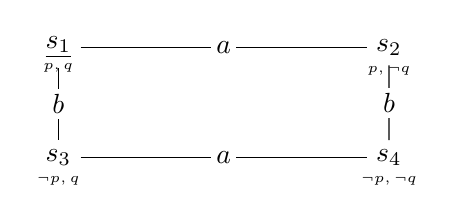
\begin{tikzpicture}[scale = 1.4, every label/.append style = {font=\tiny}]	
				\node[label={[label distance=-0.7cm]:$p,q$}] (s1) at (0,1) {$\underline{s_1}$};
				\node[label={[label distance=-0.7cm]:$p, \neg q$}] (s2) at (3,1) {$s_2$};
				\node[label={[label distance=-0.7cm]:$\neg p, q$}] (s3) at (0,0) {$s_3$};
				\node[label={[label distance=-0.7cm]:$\neg p, \neg q$}] (s4) at (3,0) {$s_4$};
	
				\path[every node/.append style={font=\fontsize{10}{0}, fill=white, inner sep=2pt}] 
					(s1) edge node {$a$} (s2) ++
					(s3) edge node {$a$} (s4) ++
					(s1) edge node {$b$} (s3) ++
					(s2) edge node {$b$} (s4);								
		\end{tikzpicture}
	} %End scaling
	\caption{A basic bisimulation contracted model.}
	\label{fig:GAexample}
\end{figure}

If we attempt to determine which sets of formulas some agent $i$ can announce in the model in Figure \ref{fig:GAexample} we can see that the set of announceable formula extensions will always be a subset of the power set of states in the model. Or more precisely, the set of announceable formula extensions for some agent $i$ in a given pointed model $\M,s$ is a subset of the power set of states in $\M$, where each set is announceable by $i$ if and only if that set follows the following rules in Definition \ref{def:extRules}.

%subset of the power set of extensions of the set of labeling formulas for the model

\begin{definition}[Rules for eliminating formulas by their extension]\hfill
\label{def:extRules}
	For any formula $\varphi$ and bisimulation contracted pointed model $\M,s$, the formula's extension in $\M$, $\ext{\varphi}_{\M}$, must satisfy the following rules in order for the formula to be announceable by some agent $i$ in coalition $G$:
	\begin{itemize}
		\item $\ext{\varphi}_\M$ must contain the actual state in our pointed model
		\item $\forall s\in\ext{\varphi}_{\M}, \forall t\rels_i s \Rightarrow t\in\ext{\varphi}_{\M}$
	\end{itemize}
\end{definition}

The reasoning behind these two rules is based on the semantics of the group announcement operators in Definition \ref{def:GALsem}, we can see that we are essentially searching for a combination of formulas which when announced, make $\varphi$ false. Because of this, having an agent announce that they know something which is false, or something they do not actually know, will simply make the public announcement trivially true. This means there is no point in checking any announcement containing such a formula, therefore the formula:

\begin{itemize}
	\item[(1)] has to be satisfied in the `actual' state of our pointed model
	\item[(2)] has to be satisfied in every state the agent is incapable of distinguishing from that `actual' state
\end{itemize}

\begin{proposition}
For every extension $\ext{\varphi}_{\M}$ that satisfies the rules in Definition \ref{def:extRules} for some agent, any formula with the same extension can be announced by that agent
\end{proposition}

From our definition of formula extensions in Definition \ref{def:ext}, the extension of a formula is simply the set of states in which this formula is satisfied. Therefore if $\varphi$ and $\psi$ share the same extension in some model $\M$, then $\M\models\varphi \leftrightarrow \psi$. From this we can further infer that $\M\models K_a\varphi \leftrightarrow K_a\psi$ for every $\psi$ with the same extension as $\varphi$


\begin{definition}[The set of announceable extensions]\hfill\\
	\label{def:annexts}
	The set of announceable formula extensions $\anns{}$ for some agent $i$, given a pointed model $\M,s$ is defined 			as the following: \\
	$\anns{i,(\M,s)} \subseteq \wp(\{\ext{\varphi}_{\M} ~|~ \varphi\in\labels{\M}\})$ where $\ext{\varphi}_\M \in 		     
	\anns{i,(\M,s)}$ iff it follows the rules in Definition \ref{def:extRules}.
	Note that since every formula in $\labels{\M}$ is only satisfied in a single state in $\states$ and every state in $\states$ satisfies exactly one formula in $\labels{M}$, $\wp(\{||\varphi||_\M ~|~ \varphi \in \labels{\M}\})$ can be simplified to $\wp(\states)$.
\end{definition}

For a more practical explanation we will apply these rules to the model in Figure \ref{fig:GAexample} for agent $a$. Using $s_1$, denoted $1$ in the next example, as the actual state of our pointed model, we start by generating the power set of states in our model and get the following:

\begin{align*}
	\wp(\states) = \{\emptyset,\{1\},\{2\},\{3\},\{4\},\{1,2\},...,\{1,2,3\},...\{1,2,3,4\}\}
\end{align*}
After applying rule (1) from Definition \ref{def:extRules}	to filter out all formula extensions not containing the actual state of our pointed model we get:
\begin{align*}
	\{\{1\},\{1,2\},\{1,3\},\{1,4\},\{1,2,3\},\{1,2,4\},\{1,3,4\},\{1,2,3,4\}\}
\end{align*}
Applying rule (2) to remove all extensions relating to formulas that $a$ does not know leaves us with:
\begin{align*}
	\{\{1,2\},\{1,2,3,4\}\}
\end{align*}

In other words, given the model in Figure \ref{fig:GAexample} agent $a$ is able to announce any given formula $\varphi$ iff $\ext{\varphi}_{\M,1} \in \{\{1,2\},\{1,2,3,4\}\}$. Therefore, $\anns{a,(\M,1)} = \{\{1,2\},\{1,2,3,4\}\}$.

An interesting thing to note here is that we can combine our labeling formulas with disjunctions to create a formula which is satisfied in any subset of the original set of states we want. So for example, in order to create a formula with the extension of $\{s_1,s_2\}$ all we have to do is put disjunctions between the labeling formulas for $s_1$ and $s_2$ such that $\varphi_{\{s_1,s_2\}} = \varphi_{s_1} \vee \varphi_{s_2}$.

If we then want to apply this to checking whether $\M,s_1 \models \dia{a}K_bp$ where $\M$ is still the model in Figure \ref{fig:GAexample} then we can see that since $\{s_1,s_2\}\in\anns{a,(\M,s_1)}$ there exists a formula extension that $a$ can announce which would eliminate $s_3$ from the model. This would cause $K_bp$ to be satisfied in the updated model and therefore satisfy $\dia{a}K_bp$.

\subsection{Generalizing the single agent case}

Expanding what we have presented so far to encompass coalitions comprised of multiple agents is actually very easy. 
When we are assessing the ability of an agent to announce something which may change the valuation of a formula, we are simply checking whether or not that agent is capable of eliminating certain states in the updated model. In other words, if we wish to assess the ability of a whole coalition, all we need to do is look at which sets of states each agent in the coalition is able to eliminate in unison.

An interesting observation to make is that an agent $i$ is always capable of eliminating any state they can distinguish from the actual state of some pointed model. This means that in order to find out which states a coalition can eliminate, we can simply take the power set of states and limit it to the combinations of states which fit the rules of Definition \ref{def:extRules}, where we slightly tweak rule 2 to the following:

\begin{definition}[The set of extensions announceable by coalitions]
	\label{def:extscoal}
	The set of announceable extensions $\anns{G,(\M,s)}$ for some coalition $G$, given a bisimulation contracted pointed model $\M,s$ is defined as the following: \\
	$\anns{G,(\M,s)} = \{\states' \subseteq \states ~|~ \forall s'\in \states', \neg\exists t\forall i\in G ~ t\rels_i s', t\not\in \states' \textrm{ and } s\in\states'\}$
\end{definition}

A candidate set $\states'\subseteq\states$ not satisfying the condition is clearly not announceable because it contains a state $s$ which no agent in the coalition can distinguish from the excluded state $t$.

\subsection{Proof of suitability}

In this section we will compare our definitions and work so far with the definitions presented by Ågotnes et al. in their paper on GAL. In their paper they describe how to check formulas of the kind $\dia{G}\varphi$ in the following manner:

\begin{definition}[Definition of $\dia{G}\varphi$ by Ågotnes et al.]
	\label{def:GALsemAagotnes}
	$\M,s\models \dia{G}$ iff there is a definable restriction $\M'' = (\states'',\rels'',V')$ of $\M$  such that $\states'' = \cap_{i\in G}C_i$ where  $C_i$  are unions of classes of equivalence for $\rels_i$ and $s\in\states''$ and $\M',s\models\varphi$
\end{definition}

Decomposing their definition we end up with $\states''$ being the intersection of the unions of some subset of each agent's equivalence relation. More specifically, for each agent $i$, we choose which equivalence classes 
should be part of that agent's union of equivalence classes $C_i$ and then check if there exists some combination of values for each $C_i$ such that restricting the set of states to the intersection of these $C_i$s gives us a model which both contains the original state $s$ and satisfies $\varphi$.

Comparing this definition to our definition of the announceable set of extensions for a coalition, we argue that our definition of $\anns{G,(\M,s)}$ defines exactly these intersections of possible combinations of $C_i$s from the definition of Ågotnes et al. If we further decompose their definition, we end up with the two following restrictions:
\begin{align}
	&S'' = \bigcap_{i\in G}C_i \textrm{ where } C_i \subseteq S, \forall s\in C_i, \eqc{s}_i\subseteq C_i \\
	&s \in S''
\end{align}

From this, we argue that our definition of $\anns{G,(\M,s)}$ incorporates the same two restrictions, in turn quantifying the set of all possible restricted sets $\states''$. Decomposing our definition the same way we did Definition \ref{def:GALsemAagotnes}, we end up with $\anns{G,(\M,s)}$ defined as the set of all subsets of $\states$, $S'$ which satisfy the following two restrictions:
\begin{align}
	&\forall s'\in S' \neg\exists t\forall i \in G, t\rels_i s', t\not\in S' \\
	&s\in S'
\end{align}

Expanding on our restriction in $(3)$, we could write it out as `if there exists a state $t$ indistinguishable by all agents from $s$, then either $t\in S'$ or $s\not\in S'$'. A simpler way of phrasing this would be to say that for every state in $S'$, the intersection of its equivalence classes for all agents in the coalition has to be a subset of $S'$. Changing (3) to fit this simpler phrasing gives us
\begin{align}
	\forall s'\in S' \cap_{i\in G}\eqc{s'}_i\subseteq S'
\end{align}

which should further clarify that combining restriction $(4)$ and $(5)$ provides the same set of possible values as $(1)$ and $(2)$. Based on this, we revise the semantics for the group announcement operators into the following:

\begin{definition}[Group announcement operators, revised]
	\label{def:GALsemV2}
	\begin{align*}
		\M,s & \models [G]\varphi \textrm{ iff }  \forall Ext\in\anns{G,(\M,s)} \textrm{ then } \M,s\models [\varphi_{Ext}]\varphi\\
		\M,s & \models \dia{G}\varphi \textrm{ iff } \exists Ext\in\anns{G,(\M,s)} \textrm{ such that } \M,s\models \dia{\varphi_{Ext}}\varphi
	\end{align*}
	where $\varphi_{Ext}$ is a formula of the form $\bigvee_{s\in Ext}\varphi_{s}$
\end{definition}

Our reason for revising these definitions is that the original definitions in \ref{def:GALsem} define satisfaction of $[G]\varphi$ by using a quantifier over an infinite set of formulas making it unfit for our goals of implementing a model checking tool. We will therefore be implementing the revised definition in \ref{def:GALsemV2} instead as the set of announceable extensions is far easier to enumerate than the set of announceable formulas. This is still equivalent to the original definition as we are simply grouping the infinite set of announceable formulas into a finite set of announceable extensions.

\subsection{Algorithm for bisimilarity check}

Using the definition of bisimilarity in Definition \ref{def:bisim} we present our recursive function for checking bisimilarity between states. Given a set of states $States$, a set of agents $Agents$ and two states $s$ and $s'$ such that $s, s' \in States$, the function (recursive bisimulation check) $rbc(s,s',States, Agents)$ determines whether $s$ and $s'$ are bisimilar is defined as Algorithm \ref{alg:rbc}.

\begin{algorithm}
\caption{Recursive Bisimulation Check}
\label{alg:rbc}
\begin{algorithmic}[H]
\Function{$rbc$}{$s,s',States,Agents$}
	\If {$s = s'$}
		\State\Return $true$
	\ElsIf{$props(s) \ \neq \ props(s')$}
		\State\Return $false$
	\ElsIf{States = $\O$}
		\State\Return $true$
	\Else
		\State $States' \gets States \setminus \{s,s'\}$
		\State $forth \gets$ \Call{$knowledgeCheck$}{$s,s',States',Agents$}
		\State $back \gets$ \Call{$knowledgeCheck$}{$s',s,States',Agents$}
		\State \Return $(forth \ and \ back)$
	\EndIf
\EndFunction
\end{algorithmic}
\end{algorithm}

The resulting algorithm is fairly similar to the logical definition, with the $props$ check being equivalent to the $atoms$ clause and the $knowledgeCheck$ function replacing the $forth$ and $back$ clauses. Note that our valuation function is flipped, going from a state to a set of propositions, rather than a proposition to a set of states. The pseudocode for the $knowledgeCheck$ function used to translate $forth$ and $back$ is shown in Algorithm \ref{alg:kc}.

\begin{algorithm}
\caption{Knowledge Check}
\label{alg:kc}
\begin{algorithmic}
\Function{$knowledgeCheck$}{$s,s',States,Agents$}
	\ForAll{$(t, Ags) \ in \ neighbours(s,Agents, States')$}
		\ForAll{$a \ in \ Ags$}
			\State $hasMatching \gets false$
			\ForAll{$(t', Ags') \ in \ neighbours(s', Agents, States')$}
				\If{$a \in Ags'$ and \Call{$rbc$}{$t,t',States',Agents$}}
					\State $hasMatching \gets true$
					\State $\mathbf{break}$
				\EndIf
			\EndFor
			\If{!hasMatching}
				\State\Return $false$
			\EndIf
		\EndFor	
	\EndFor
	\State \Return $true$ 
\EndFunction
\end{algorithmic}
\end{algorithm}

Comparing our algorithm to the original definition of bisimilarity the main point of interest is how it is finite, since for each recursive call to $rbc$ we prevent the two current states from being checked again, meaning that at some point the algorithm is guaranteed to halt. The function $neighbours$ used in the $knowledgeCheck$ function simply returns a set of tuples for each state visible from $s$ and the set of agents it is visible to, limited to states in $States$.

\subsection{Smallest bisimilar structure}

Building on the previous algorithm, the next step is using it to create an algorithm for constraining a model to one of its smallest bisimilar structures, by filtering out all bisimilar states. While we normally would not need to worry about which states are filtered, as we are generating a checking log to visualize the checking process for our users, we wanted to avoid having the `actual' state of our pointed model filtered out. As such, we simply make sure that the actual state lies first in our set of states when calling $bisimContract$ in our application. 

\begin{algorithm}
	\caption{Bisimulation contraction}
	\label{alg:bisimContract}
	\begin{algorithmic}
		\Function{$bisimContract$}{$States, Agents, Edges$}
			\State $bisimMap \gets Map<State, State>$
			\ForAll{$(state) \ in \ States$}
				\ForAll{$(otherState) \ in \ States \setminus (state \ \cup \ keys \  in \ bisimMap) $}
					\If{\Call{$rbc$}{$state, otherState, States, Agents$}}
						\State \Call{$bisimMap.put$} {$otherState, state$}
					\EndIf
				\EndFor
			\EndFor
			\State $CS \gets States \ \setminus \ (keys \ in \ bisimMap)$
			\State $CE \gets \{ e \in Edges ~|~ e.state1 \in CS \ and \ e.state2 \in CS\}$
			\State $contractedModel \gets (CS, Agents, CE)$
			\State \Return $contractedModel$
		\EndFunction
	\end{algorithmic}
\end{algorithm}

\subsection{Enumerating the set of announceable extensions}

As we have now laid the groundwork of formulating how we can compute bisimulation contractions of models, we can move on to presenting how we can generate the set of announceable extensions. For this we will be using the definition of announceable extensions presented in Definition \ref{def:extscoal}. While Ågotnes et al.'s definition in \ref{def:GALsemAagotnes} is more compact, our definition more closely resembles its pseudocode translation.

\begin{algorithm}
	\caption{Generating a coalition's set of announceable extensions}
	\label{alg:genAnnExts}
	\begin{algorithmic}
		\Function{$genAnnExts$}{$contractedModel, actState, coalition$}
			\State $states \gets contractedModel.states$
			\State $extensions \gets \wp(states)$
			\ForAll {$extension ~ in ~ extensions$}
				\If {$actState \not\in extension$}
					\State remove $extension$ from $extensions$
				\Else
					\ForAll {$state$ in $extension$}
						\State $eqClass \gets $\Call{$genEqClass$}{$state, states, coalition$}
						\ForAll {$eqstate$ in $eqClass$}
							\If {$eqstate \not\in extension$}
								\State remove $extension$ from $extensions$
								\State $\mathbf{break}$
							\EndIf
						\EndFor
					\EndFor
				\EndIf				
			\EndFor
			\State \Return $extensions$
		\EndFunction
	\end{algorithmic}
\end{algorithm}

As can be seen, the algorithm for generating the set of announceable extensions boils down to generating the power set of states in the model, i.e. the set of all possible extensions, and then filtering it according to the rules in Definition \ref{def:extRules}. The $genEqClass(state, agents)$ function used is mostly identical to the $neighbours$ function used previously, except it returns the list of states that the coalition as a whole considers indistinguishable from the input state. 

Now that we have not only our bisimulation contracted model, but also a way to generate all of the announceable formula extensions for any coalition, describing the algorithm for checking group announcement formulas becomes straightforward. As these extensions are really just stand-ins for some announcement made by the agents as per the original definition in Definition \ref{def:GALsem}, we can also regard them as constraints on our model. Going by our revised definition of the semantics behind the group announcement operator from definition \ref{def:GALsemV2}, all our algorithm needs to do is to check whether all of the constrained models we get from applying these constraints to our bisimulation contracted model satisfy the post condition of the group announcement. As such, we translated the semantics of the group announcement operator into the following checking function, shown in Algorithm \ref{alg:checkGroupAnn}.

%Discuss optimizations in regards to non-epistemic formulas not changing valuation through announcements\\
\begin{algorithm}
	\caption{Check function for group announcement operator}
	\label{alg:checkGroupAnn}
	\begin{algorithmic}	
		\Function{$check_{[G]\varphi}$}{$state, innerForm, model, coalition$}
		\State $contractedModel \gets$ \Call{$bisimContract$}{$model$}
		\State $extensions \gets $\Call{$genAnnExts$}{$contractedModel, state, coalition$}
		\ForAll {$extension$ in $extensions$}
			\State $constMdl \gets$ \Call{$constrainMdlBy$}{$contractedModel, extension$}
			\State $extSatisfiesForm \gets $ \Call{$check$}{$state, innerForm, constMdl, coalition$}
			\If{$!extSatisfiesForm$}
				\State \Return $false$
			\EndIf
		\EndFor
		\State \Return $true$
		\EndFunction
	\end{algorithmic}
\end{algorithm}

Like we previously mentioned we here make sure the set of states passed to $bisimContract$ starts with the actual state we're checking our formula in, in order to simplify the visualization of our checking process. It should also be mentioned that the $check$ function that gets called is implemented as an abstract function overridden by each operator in our system and that Algorithm \ref{alg:checkGroupAnn} only shows the implementation for the group announcement operator. The $constrainMdlBy$ function used here is merely a special case of updating a model through announcing the set of states directly instead of announcing a formula and constraining our model to the set of states that satisfy the given formula. 

%\todo{Show algorithms for checking conjunctions, knowledge and public announcements}

Now that we have presented our algorithm for checking group announcements, we will additionally present our checking algorithms for a few of the simpler operators as well. Starting out, we present Algorithm \ref{alg:checkConj} for checking conjunctions. As all of the non-epistemic operators can be checked in similar fashion with only minor tweaks to the algorithm, we will be skipping the rest of them and instead move on to the knowledge operator. 

\begin{algorithm}
	\caption{Check function for the conjunction operator}
	\label{alg:checkConj}
	\begin{algorithmic}
		\Function{$check_{\varphi\wedge\psi}$}{$state, leftForm, rightForm, model$}
		\State $leftSatisfied \gets $ \Call{$check$}{$state, leftForm, model$}
		\If{$leftSatisfied$}
			\State \Return \Call{$check$}{$state, rightForm, model$}
		\Else
			\State \Return $false$
		\EndIf
		\EndFunction
	\end{algorithmic}
\end{algorithm}

Algorithm \ref{alg:checkKnowledge} describes how we check knowledge in our model checker. The $getIndishStates$ function we use here returns the set of states an agent considers indistinguishable from the given state, which is then looped over as we check whether the `inner' formula is satisfied in all these indistinguishable states.

\begin{algorithm}
	\caption{Check function for knowledge operator}
	\label{alg:checkKnowledge}
	\begin{algorithmic}
		\Function{$check_{K}$}{$state, innerForm, agent, model$}
		\State $indistinguishableStates \gets $ \Call{$getIndishStates$} {$state, agent$}
		\ForAll {$indishState$ in $indishtinguishableStates$}
			\If {!\Call {$check$}{$indishState, innerForm, model$}}
				\State \Return $false$
			\EndIf
		\EndFor
		\State \Return $true$
		\EndFunction
	\end{algorithmic}
\end{algorithm}

Finally, we also present Algorithm \ref{alg:checkPubAnn} for checking public announcements. Note that we also check if the announcement is truthful and immediately return true if this is not the case as false announcements would lead to contradictions per the semantics of public announcements.

\begin{algorithm}
	\caption{Check function for public announcements}
	\label{alg:checkPubAnn}
	\begin{algorithmic}
		\Function{$check_{[\varphi]\psi}$}{$state, announcement, innerForm, model$}
		\If {!\Call {$check$} {$state, announcement, model$}}
			\State \Return $true$
		\EndIf
		\State $updStates \gets List <State>$
		\ForAll {$currState$ in $model.states$}
			\If {\Call {$check$}{$currState, announcement, model$}}
				\State $updStates.add(state)$
			\EndIf
		\EndFor
		\State $updEdges \gets List <Edge>$
		\ForAll{ $edge$ in $model.edges$}
			\If {$edge.state1 \in updStates$ and $edge.state2 \in updStates$}
				\State $updEdges.add(edge)$
			\EndIf
		\EndFor
		\State $updModel \gets$ \Call {$updateModel$}{$updStates, updEdges, agents$}
		\State \Return \Call {$check$}{$state, innerForm, updModel$}
		\EndFunction
	\end{algorithmic}
\end{algorithm} \newpage
%%Test formulas for Muddy Children:
%[ma|(mb|mc)][(!KA(ma))&((!KB(mb))&(!KC(mc)))]KB(mb)
%

\section{Model checking}\label{sec:impl}


\subsection{Model checking for Group Announcement Logic}



\subsection{Complexity of the model checking problem}

In this section we will be discussing and analyzing the run-time complexity of this model checking problem based on the algorithms we have presented so far.

For the discussion we will only be looking at the complexity of the group announcement operator and its related challenges, as the other operators of GAL are all fairly trivial to check, being O(1) operations, with the exception of the knowledge operator being O(n), where n is the number of states indistinguishable to the one we are checking the formula in.

\subsection{Generating examples}

\question{Flytte til implementasjon?}

In this section we will discuss the topic of generating examples which prove why or why not a formula holds in a given model. As our motivation behind this project was to create a learning tool to help new logicians understand how the semantics of GAL work, being able to generate examples which highlight interesting properties of our models is highly important. As such, MCGAL was designed from the ground up to be able to trace its steps through the model checking process so that it can also display each step of this process in an intuitive manner. The program therefore creates a log entry each time it checks an operator against a specific state in the model, keeping track of sub-formulas and formula depth as it goes through the operators. The reason behind also keeping track of sub-formulas and formula depth in the logs is to create a more tree-like structure, so that the user can more easily skip through chunks of the process that might not be particularly interesting, allowing them to for example view each state the tool checks against a particular K-operator, or even skip through each of the possible updated models a coalition can reduce a model to through their announceable extensions.

\begin{figure}[H]
	\label{fig:basicGalChecking}
	\caption{Checking a basic group announcement formula in MCGAL}
	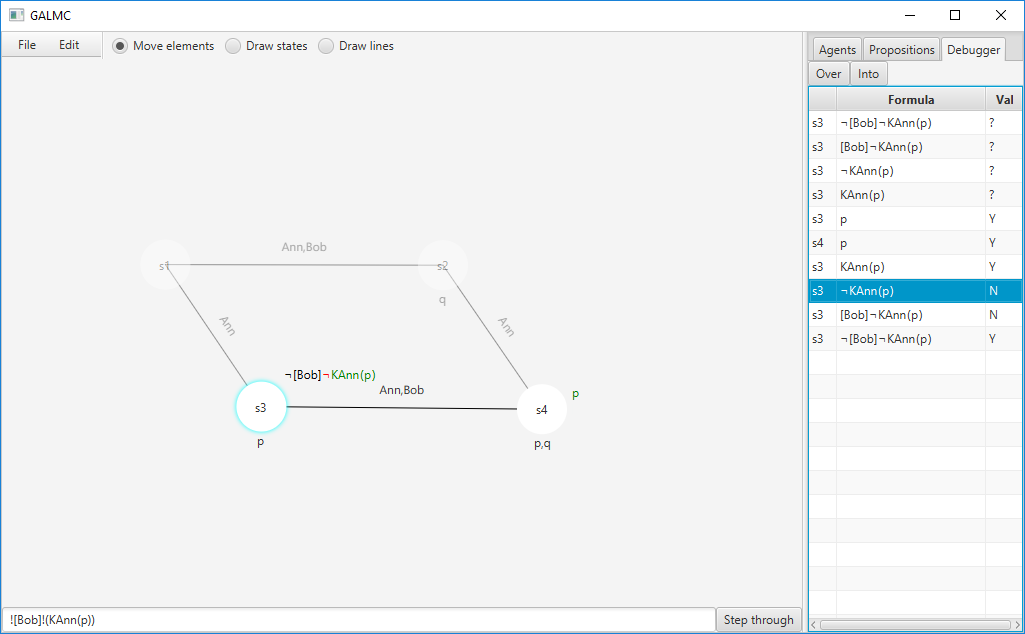
\includegraphics[width= \textwidth]{MCGALBasicChecking.png}
\end{figure}

As the tool provides a view of the model, it also updates this view by highlighting what the model it is currently checking against looks like, by graying out any states that have been filtered out by a model update, such as each formula extension a coalition can announce, which is what is being displayed in Figure \ref{fig:basicGalChecking}. In this example, we are checking state s3 against the formula $\neg [Bob]\neg KAnn[p]$ translating to: 'It is not the case that Bob is unable to make Ann know $p$' or more simply in its dual form: 'Bob is able to make Ann know p'. In the figure we can see that as Bob is able to reduce the model to only states where $p$ holds, Ann also trivially knows $p$ in this updated model, satisfying our original formula. In our somewhat trivial example, the tool ended up only trying a single model as it only had to find a single extension that made the formula true. If we were to check an unnegated group announcement formula, it would have to check every possible formula extension announceable by the given coalition, but it would also visualize all of these updated models until it finds one where the formula does not hold, giving the user insight into the coalitions capabilities. Note that the previous example could also have been made easier by rewriting the formula as $\dia{Bob}KAnn[p]$, but unfortunately the tool does not (yet) support diamond operators. 
 \newpage
\section{GALMC}\label{sec:impl}

In this chapter we will present our own implementation of a model checker for Group Announcement Logic called \cname{} and describe its inner workings. \cname{} is intended to be an educational tool which aids students in learning epistemic logic in a more visual manner. Therefore, while most other model checking utilities such as DEMO \cite{JanvanEijck} stick to answering the user's queries with simple yes and no answers, \cname{} goes beyond that by showing them not just whether their formulas hold, but also visualizes why and provides the user with an easier, visual way of drawing models almost as they would on paper or blackboard. The reasoning behind this was that by allowing the user to manipulate the model through a simple click-and-drag interface and seeing how it can affect the valuation of various formulas, they might gain a deeper understanding of the semantics involved.

One of the big questions that needed to be answered when building \cname{} was how to not just present and visualize these highly abstract models, but also allow the user to manipulate them in a way that would be intuitive and easy to grasp. As I had previously used a tool called JFLAP\footnote{www.jflap.org} with great success when teaching students as a TA about Turing machines and finite state automata (FSAs) I ended up drawing most of my inspiration from it when drawing up my initial sketches for how I imagined my own tool might look. While my own experience with JFLAP is mostly limited to visualizing, editing and playing with Turing machines and finite state automatas, it is a fairly sophisticated package of graphical tools covering also covering many other concepts of formal languages and automata theory. JFLAPs editor is relatively simplistic, but it still helped my own and my students' understanding of FSAs tremendously by allowing us to interact and play with what is otherwise a really abstract concept and as such, I wanted to see if I could create a similarly potent learning aid for epistemic logic. 

\begin{figure}[H]
	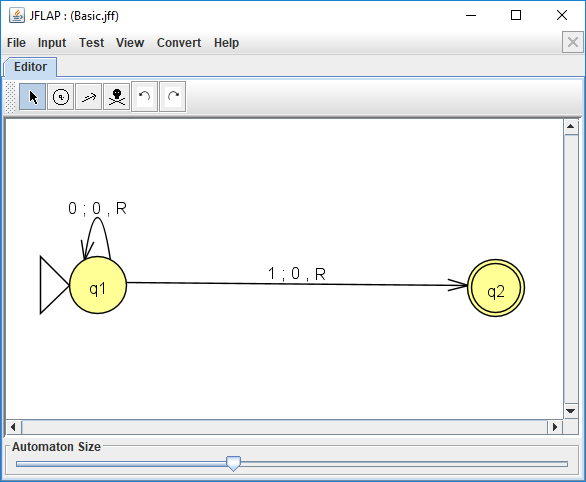
\includegraphics[width= \textwidth]{JFLAPbasicIllustration.PNG}
	\caption{A basic two-state turing machine}
	\label{fig:JFLAP_basic illustration}
\end{figure}

%When I took the same course myself the year before I became a TA in it, most of the students, myself included found Turing machines to be a really hard and abstract concept to grasp as we were simply explained how they worked and then instructed to write instructions that would perform certain basic tasks using pen and paper alone. Obviously, this left us without any way to check whether or not our 

While I could have created a simpler non-graphical model checking tool for GAL similar to DEMO, I wanted to create something more powerful that could help visualize epistemic logic the same way that JFLAP visualizes Turing machines. My justification is that although a similar non-graphical tool would probably have helped me teach my students how FSAs and Turing machines work as well, I highly doubt it would have been anywhere near as effective without being able to visualize the `how's and `why's and instead only gave `yes' or `no' answers to our queries in the same manner that most model checking utilities do. 
%Learning benefit

\subsection{Visualization of Kripke structures}
%Visualization of Turing machines vs kripke stuctures
%Both have states, transitions vs indistinguishability, tape of input vs formula to traverse and check
Although finite state automatons and epistemic logic might initially seem relatively far detached, the Kripke structures we use share a fair few similarities to FSAs that made me realize I could visualize our models in almost the same manner as JFLAP does its automata. For instance, they both consist of a set of states, and while FSAs and Turing machines have transition rules, and Kripke models have an indistinguishability relation, they can both be visualized as edges in a graph where the nodes are our states. Whereas JFLAP labels its edges with the each transition rule, we label ours with the set of agents that considers our pair of states indistinguishable and additionally label each state with the set of propositions that hold in it. We present our tool visualizing a basic model in Figure \ref{fig:basicModelVis}.


\begin{figure}[H]
	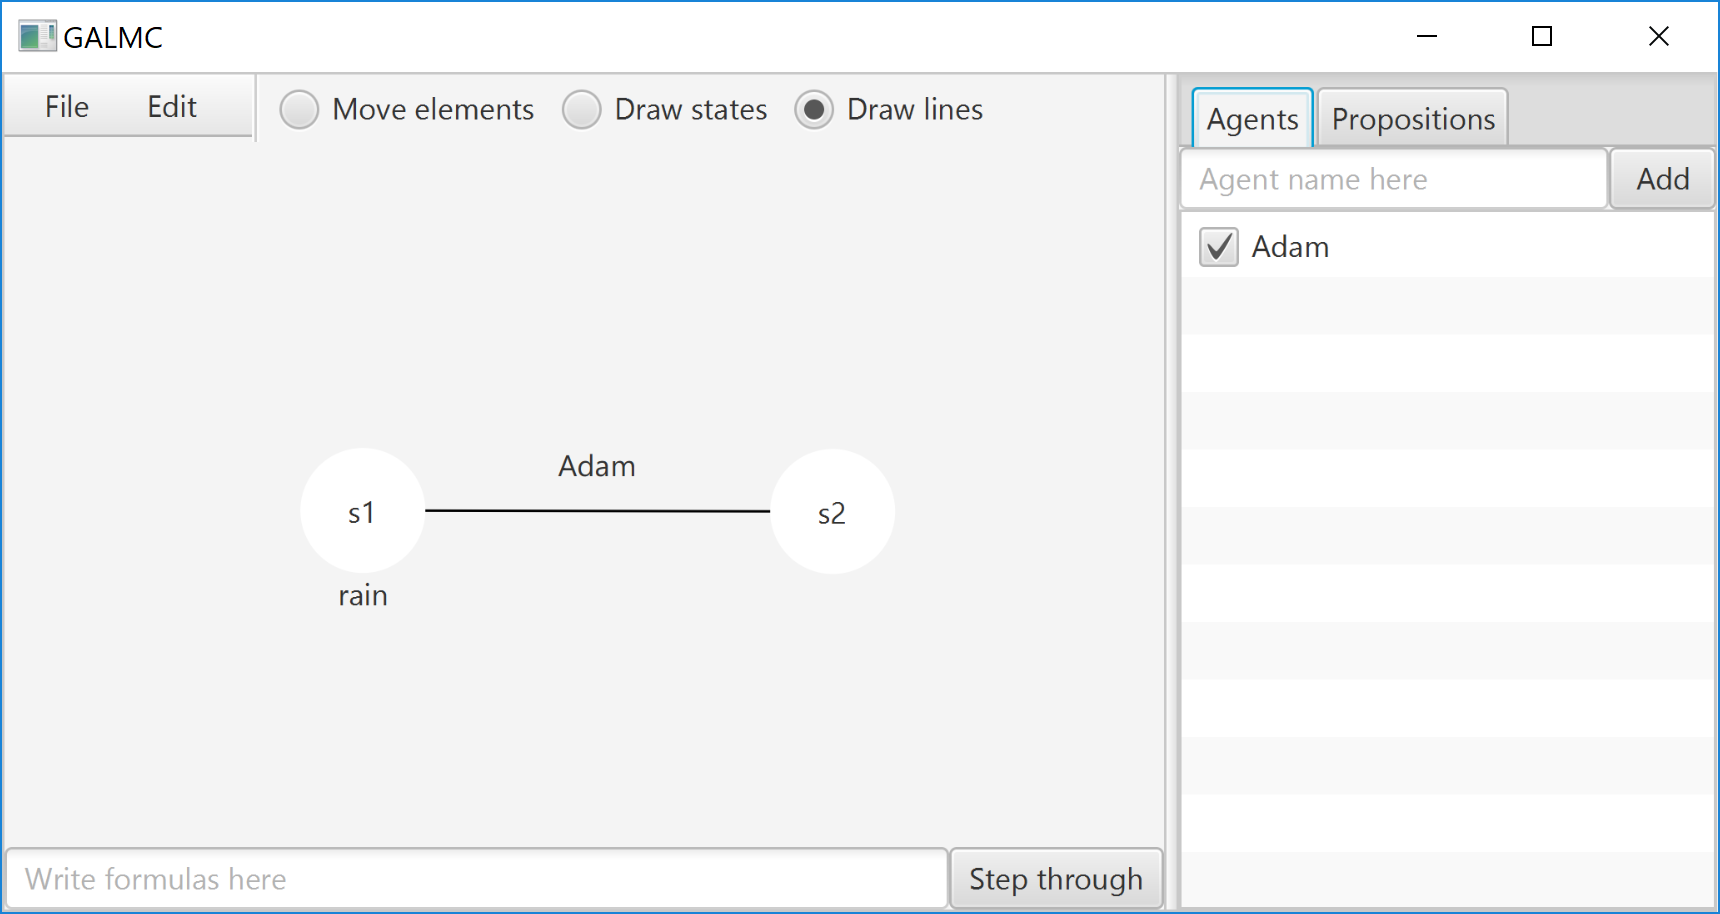
\includegraphics[width= \textwidth]{BasicModel.png}
	\caption{A basic model, visualized in \cname}
	\label{fig:basicModelVis}
\end{figure} 

%Mention basic usage, how one draws models, example blackboard, simple, intuitive, easy
Figure \ref{fig:basicModelVis} shows how \cname{} visualizes the basic model we introduced in Figure \ref{fig:basicEM} and as can be seen, the UI of \cname{} is fairly close to that of JFLAP, in order to capture its simplicity. The reason for this being to enable the user to draw models in a fashion as close to how they would with pen and paper as possible so that the interface feels `natural' and intuitive to someone with little previous experience with Kripke structures. As such, the editor was made to be as clean as possible, consisting of only three main tools; one for selecting and moving elements, one for drawing new states and one for creating edges between them. Additionally, the editor provides two side panels for managing the lists of properties and agents in our models; the proposition panel for selecting which propositions should hold in newly drawn states or to update existing ones, and the agent panel which allows the user to similarly determine which agents' equivalence relations should be updated when manipulating edges.

\subsection{Checking formulas}

After the user creates their model, the next step is to start checking formulas against it. One trade-off that had to be made here was whether or not to stick to the original symbols for the various operators in our language or to come up with replacements which are easier to type in. As most of the logical symbols used to represent the various operators in GAL cannot be found on normal keyboards, naturally making them vary hard for the user to input, \cname{} replaces them with more easily accessible replacements. By the assumption that most of \cname's userbase would be at least somewhat familiar with programming, these replacements were lifted from symbols used to represent boolean operators in programming, such as replacing $\vee$ and $\wedge$ with $|$ and $\&$ for disjunctions and conjunctions respectively, as they can basically be seen as `(inclusive) or' and `and'. A full list of operators and their replacement symbols are displayed in Table \ref{tbl:symbolReplacements}\footnote{This list of replacements and a more complete user guide is also available from https://github.com/AndersKaareEide/MCGAL/wiki}. Note that while announcements are identical to how they are in GAL, the curly braces around the set of agents in group announcements were dropped to save the user the effort of typing them in. The knowledge operator is fairly similar, except that \cname{} forces agent names to start with an upper-case letter and that the parentheses around the known formula are required. The reason behind these changes was partly to be able to make it easier for the user to tell names of agents apart from propositions in more complex formulas (\cname{} forces agent names to be capitalized, whereas propositions have to be lower case). That said, the editor translates any formula the user types in back into proper legal formulas when displaying them, making it easier for the user to connect \cname's representations with other material.

%the tool less confusing to use, once the user gets familiar with the tool and the logic itself \footnote{For a more to the point user manual, see: https://github.com/AndersKaareEide/MCGAL/wiki}.

% Uppercase agent name, easier to tell props from agents?
% but it also ended up making the parser a lot simpler to write, which will be presented and discussed a later section

\begin{table}[H]
\centering
%\resizebox{\textwidth}{!}{%
\begin{tabular}{@{}lcc@{}}
\toprule
Operator           & Logical symbol & Replacement     \\  \midrule
Negation           &       $\neg$         & !               \\
Conjunction       &      $\wedge$          & $\&$              \\
Disjunction        &    $\vee$        & $|$               \\
Implication        &       $\rightarrow$       & -\textgreater{} \\
Knowledge         &        $K_{ann}\varphi$        & $KAnn(\varphi)$            \\
Announcement   &       $[\varphi]\psi$         &  $[\varphi]\psi$     \\
Group Announcement &  $[\{ann,bob\}]\varphi$  & $[Ann,Bob]\varphi$ \\ \bottomrule
\end{tabular}%
%}
\caption{Table of operators and their symbols in \cname{}}
\label{tbl:symbolReplacements}
\end{table}

%Include BNF as table? Save it for ANTLR section

%Checking formulas, visualize which states in our model satisfy the given formula
%Mention interactive formula display with subformulas

When the user finishes typing in their formula, the tool checks their formula against each state in their model and colors each state based on whether or not the user's formula is satisfied in that state. However, in addition to translating the user's input into a legal formula and showing which states of the model satisfy the formula, \cname{} also lets the user hover over parts of their original formula in order to check the valuation of its subformulas, which can be seen in Figure \ref{fig:labelHover} (Note the mouse cursor over the `clouds' proposition). This enables the user to quickly break formulas apart and see how their various subformulas change the valuation of their containing formula. It also helps visualize the semantics behind each operator in our language in a manner that makes the logic more enjoyable to learn. 

\begin{figure}[H]
	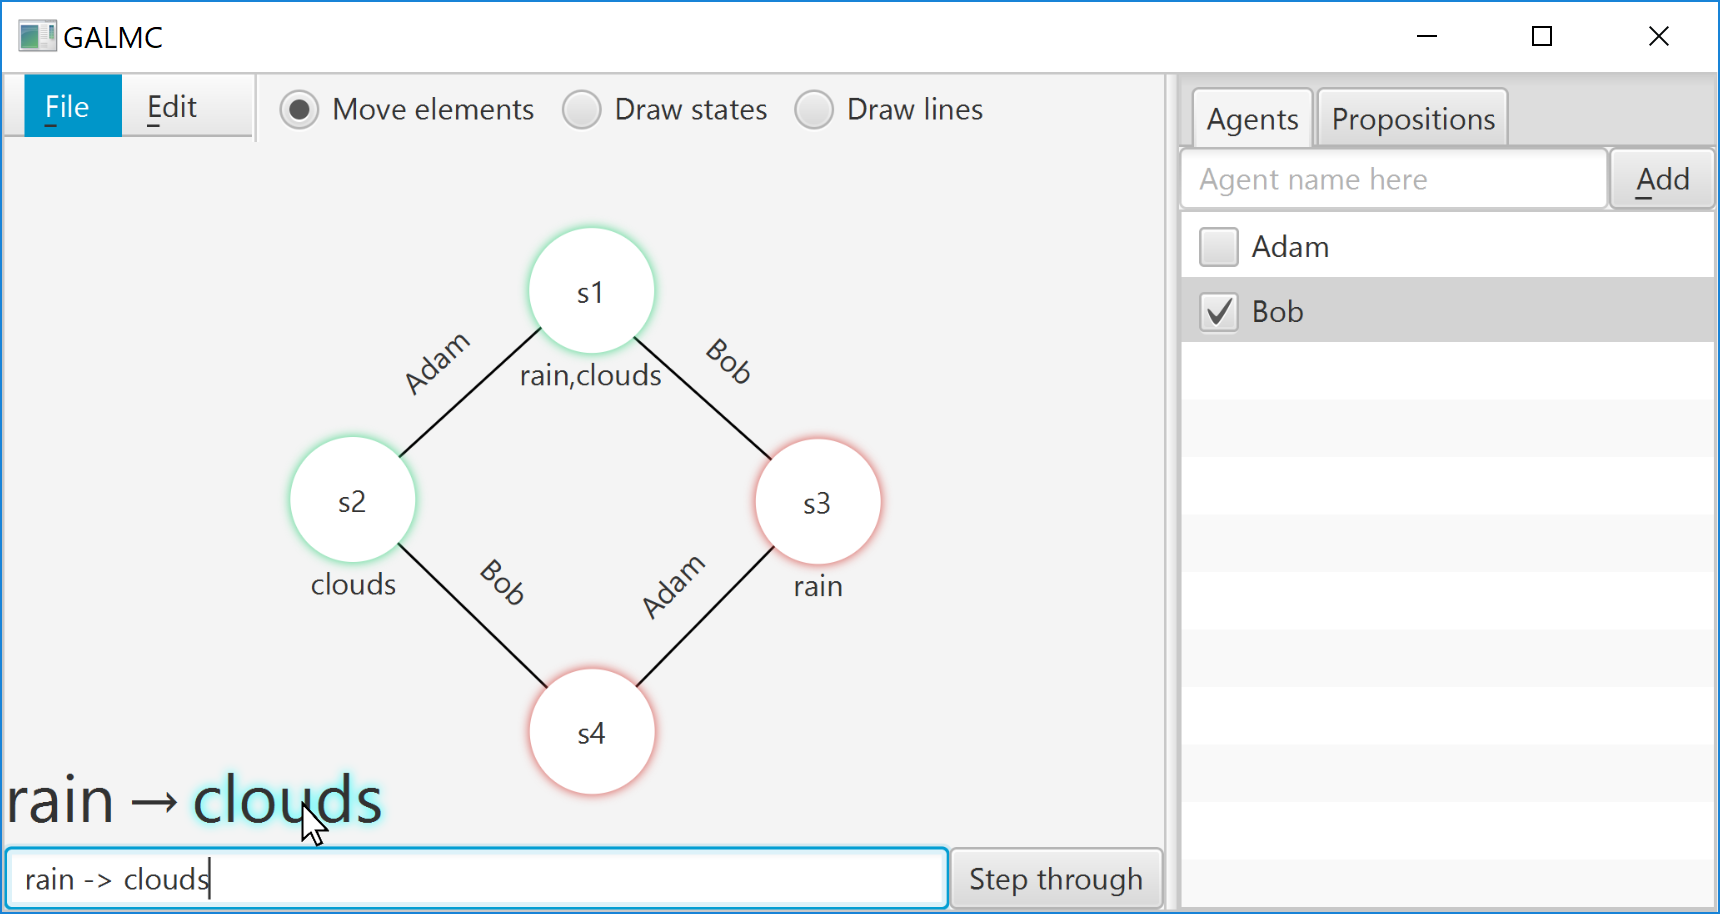
\includegraphics[width= \textwidth]{LabelMouseOver.png}
	\caption{Illustration of mousing over interactive formula display}	
	\label{fig:labelHover}
\end{figure}


\subsection{Visualizing the checking process}

One of JFLAP's most powerful features however, is its ability to step through your automatons. As you present your Turing machines in JFLAP with a set of input, the tool also allows you to step through the program of your machine one instruction at a time, while also visualizing how it manipulates the contents of its input and which state the machine is currently in. Obviously this feature is remarkably useful in showing how the user's machines operate, letting students debug their instruction sets in almost the same manner they would debug a program in a high level programming language. As such, it not only makes Turing machines and FSAs much easier to grasp, but it also makes getting them to work correctly a far less frustrating process.

Naturally, \cname{} having a similar feature, a way to visualize the process behind checking each operator in the user's formula the same way that JFLAP shows each instruction being executed and the effects of doing so would greatly improve its usefulness. This is why the tool keeps a log of each check the tool makes when evaluating a formula, logging not just the operator being checked, but also its current valuation, if known, and which state it is being checked in. Continuing with the model from our previous figure, Figure \ref{fig:stepperBasic} shows us using our tool to generate a log of how the program checks the given formula against a specific state. From this, the user can get a fully reproducible guide they can follow when checking other formulas on their own, which would be quite helpful in learning how the operators work. The user can also step forwards or backwards through this process at any time by either clicking the step they want to skip to, or browsing with the arrow keys. 

Note that in addition to this log, the program also visualizes which (sub)formulas are being checked against the various states as colorized labels that change color as the user steps through their formula based on the valuation of the operators the labels represent. 

\begin{figure}[H]
	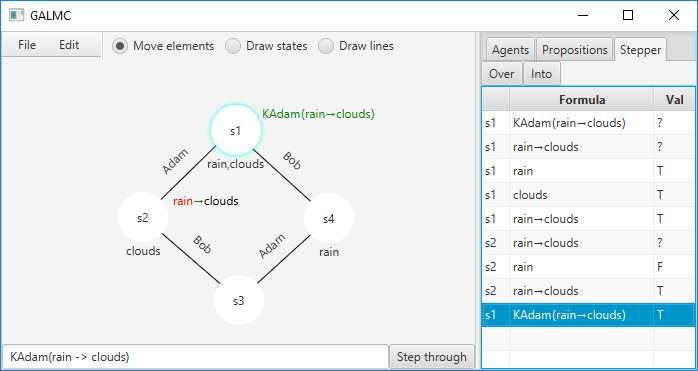
\includegraphics[width= \textwidth]{SteppingBasicExample.png}
	\caption{Illustration of using stepping functionality in \cname{}}
	\label{fig:stepperBasic}
\end{figure}


Returning to our previous comparison between the stepper in JFLAP and our adaptation for GAL, there is still an interesting challenge. While the instruction sets and states of a Turing machine are static, the epistemic models we use in dynamic epistemic logic are naturally quite dynamic, and can be updated based on public announcements in PAL or more complexly, group announcements in GAL. \cname{} represents these model updates by graying out the states and edges that were removed by the update and to update which states should be `hidden' based on which branch in the tree-like structure of the original formula the user is currently stepping through. Naturally, the tool also supports formulas with multiple announcements nesting them in any fashion the language allows, always visualizing the relevant sub-model that formulas are being checked against, an example of which can be seen in Figure \ref{fig:stepperUpdates}. Note that \cname{} also generates formula labels for which subformulas under knowledge or announcement operators have been checked in the various states, so that the user can immediately see why for example, an agent does not know something, or why a state has been filtered out in a model update.

\begin{figure}[H]
	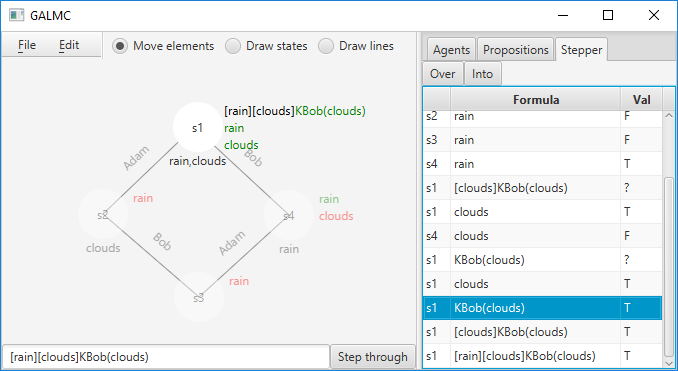
\includegraphics[width= \textwidth]{SteppingChainedAnnouncements.png}
	\caption{Visualization of the effects of chained public announcements in \cname{}}
	\label{fig:stepperUpdates}
\end{figure}
 

%Innholdsliste:

	%	Likheter i stepping over teip med input vs stepping over operatorer i formel, vise endringer i valuering i 'sanntid' på samme måte som teipen til JFLAP 
%Vis mer avansert eksempel med public announcements og modell-oppdateringer
%Vis eksempel med group announcements og hvordan verktøyet visualiserer de ulike strukturene koalisjoner kan begrense den orginale modellen til
	%	Muligens visualisere kunnskap de dicto vs de re? Må finne enkelt eksempel som ikke blir horribelt rotete i så fall


%Mention deviation from logic here? Flipped valuation function, 

\subsection{Visualizing group announcements}

Now that I have presented most of the tool I have created and how it solves the various challenges of visualizing the process of checking formulas containing the other operators in our language, it is time to discuss group announcements. As the motivation behind creating \cname{} was to create a learning tool that could help new logicians understand how the semantics of GAL work, being able to generate examples which highlight interesting properties of our models is highly important. As such, \cname{} was designed from the ground up to be able to trace its steps through the model checking process so that it can also display each step of this process in an intuitive manner, which can be seen in our previous figures. Elaborating on the logging process mentioned before behind this tracing, the tool also keeps track of subformulas and formula depth as it goes through the operators. The reason behind keeping track of this in the logs was to create a more easily navigable tree-like structure, as the number of steps required to check a formula containing group announcements can quickly explode. Because of this, \cname{} must give the user the ability to skip through chunks of the process they might not be particularly interested in. This tree-structure allows them to for example view each state the tool checks against a particular knowledge operator, or even skip through each of the possible updated models a coalition can reduce a model to through their announceable extensions, without having to step through the checking of the inner formula every time. 
 
\begin{figure}[]
	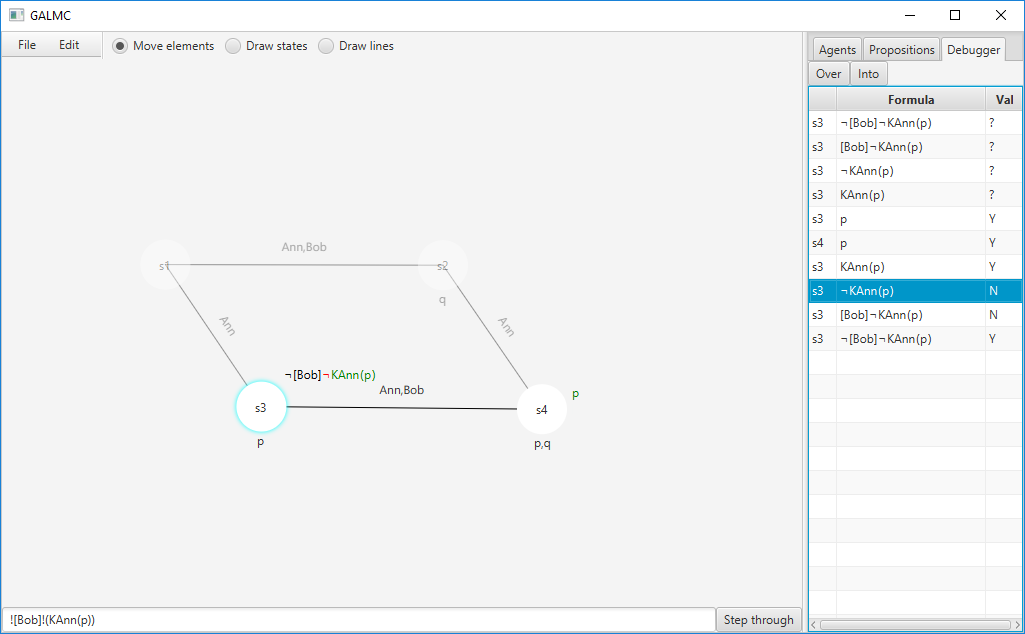
\includegraphics[width= \textwidth]{MCGALBasicChecking.png}
	\caption{Checking a basic group announcement formula in MCGAL}
	\label{fig:basicGalChecking}
\end{figure}

%\todo{Flette inn med resten av det over}

As the tool provides a view of the model and keeps track of what the model it is currently checking against looks like, it can also visualize the effects of announcing multiple different formulas. This means the tool can also visualize the result of constraining the model to the various formula extensions a coalition can announce, which is what is being displayed in Figure \ref{fig:basicGalChecking}. In this example, we are checking whether the formula $\neg [Bob]\neg K_{Ann}[p]$ holds in state s3 of our model. The formula roughly translates to: `It is not the case that Bob is unable to make Ann know $p$' or more simply in its dual form: `Bob is able to make Ann know p'. From the visualization of our model in Figure \ref{fig:basicGalChecking} we can see that since Bob is able to reduce the model to only states where $p$ holds, Ann also knows that $p$ holds in this updated model, satisfying our original formula. In this simple illustrative example, the tool ended up only having to try announcing a single formula extension before it found an extension that made our original formula true. If we were to check a more complex formula however, it might end up checking many different announcements, each generating a different updated model after its announcement which the tool will helpfully visualize, giving the user insight into a coalition's capabilities. 

%Note that the previous example could also have been made easier by rewriting the formula as $\dia{Bob}K_{Ann}[p]$, but unfortunately the tool does not (yet) support diamond operators. 

Last, but certainly not least, \cname{} also facilitates saving and loading of models. As our tool is intended to be used in educational settings, making lecturers able to create exercises for their students is highly valuable. One example of such usage would be creating and handing out an incomplete model, where the students would have to `complete' the model by either adding states or changing the indistinguishability relations for their agents in order to give this model some specific property. The lecturer could then load the models that their students have handed in to verify them. 

%As I used a similar approach to great success when introducing JFLAP to my students while teaching them automata theory and turing machines, I know how useful this feature can be. As such I wanted to make sure that my own tool could be used the same way.

%Saving / loading, distribuering av eksempler
%Oppgaver som kan gis ut, delvise modeller som skal fullføres av studenter og leveres inn

%Figure \ref{fig:debugExmpl} shows a screenshot of \cname{} in action, where the user is stepping through the process of checking a specific formula against a state in their model, having the tool visualize whether or not their formula holds. It also shows how the application breaks down epistemic formulas into sub-formulas and displays them next to each state they have to be checked in. Additionally, the application also visualizes the current valuation of each operator and proposition in the formula as you step through the checking process, as can be seen from the red and green parts of the formulas being checked, as well as the Val (valuation) column in the debugger tab. 

%Something something easier to show if we supported formula templates, future work
%Highlight difference between being able to achieve something and knowing that you are able to achieve something


%* Discuss how formulas are interpreted / parsed into tree-structures where each the nodes themselves 'contain' definitions for the semantics behind the logical connective they represent, based on their class.
%* Refer back to previously presented algorithms when discussing recursive checking function
%* Refer back to background chapter when discussing why the problem is interesting when presenting artifact.
%* Model checking often limited to yes / no questions, discuss added value by transcending boolean 

%JFLAP, a tool previously used here at our faculty to teach students how turing machines and finite state automatas work.


%Splitte opp i delkapitler? Sjekking av EL, sjekking av DEL, sjekking av GAL?

%Innholdsliste:

%Recap motivasjon
%Forklar hvorfor grensesnittet ble som det ble, inspirasjon fra JFLAP ect
%Anekdote rundt bruken av JFLAP 
	%Nytte for studenter
%Introduksjon til visualisering, vis basics
	%Trekke sammenligninger mellom visualiseringen av Kripke og FSAer
%Diskuter tegning av modeller, tilstander, kanter og agenter
	%Grunngi tegnemåte og andre avgjørelser iht UI, sidepaneler, editor-'moduser'
%Nevn håndtering av props og agentlister

%Vis eksempler på sjekking av basic formler
%Forklar innlesing av formler
%Diskuter forskjeller mellom innskreven form vs logiske symboler (enklere å skrive inn)
%Forklar hva som skjer, først sjekk hvilke states i modellen
%Nevn interaktivitet gjennom sjekke subformler ved å muse over

%Diskuter motivasjon og hensikt bak stepping-funksjonalitet
	%	Sammenlign med stepper i JFLAP
	%	Mer avansert enn JFLAP, FSA samme sett states, DEL har modelloppdateringer, kan visualiseres
	%	Likheter i stepping over teip med input vs stepping over operatorer i formel, vise endringer i valuering i 'sanntid' på samme måte som teipen til JFLAP 
%Vis basic eksempel på hvordan verktøyet presenterer steg-loggen
%Vis mer avansert eksempel med public announcements og modell-oppdateringer
%Vis eksempel med group announcements og hvordan verktøyet visualiserer de ulike strukturene koalisjoner kan begrense den orginale modellen til
	%	Muligens visualisere kunnskap de dicto vs de re? Må finne enkelt eksempel som ikke blir horribelt rotete i så fall

 \newpage
\section{Implementation details}\label{sec:impl}

In this chapter we will discuss the various tools and technologies that were used to create our tool, including, but not limited to; choice of programming language, frameworks and libraries and discuss why these were selected.

Starting off with the programming language we went with, our choice was Kotlin. Kotlin is a relatively new language which runs on the Java virtual machine\footnote{https://www.java.com/en/download/} (JVM) that has gotten a lot of attention in the recent years after Google announced they were making it an official language for Android development during their I/O conference back in 2017\cite{KotlinGoogleIO2017}. While the language has since `branched out' with JavaScript transpilers and a native compiler, letting developers target different platforms, one of the main strengths of the language is that despite being relatively young, it is able to tap into the vast number of libraries and tools written for the JVM by compiling down to Java-bytecode, allowing for full interoperability with Java. Among the other benefits of the language's relatively young age, is that it has been able to draw inspiration from other modern giving it features such as type inference, string interpolation and default values. This means that lends itself very well towards writing functional code despite being object oriented, through shorthands for lambda expressions, support for proper function types and distinctions between mutable and immutable structures and variables. As an added bonus, the language is also backed heavily by JetBrains, well known for their suite of IDEs and plugins such as IntelliJ, PyCharm and ReSharper, so the language also has first-class tooling support, making it easy to pick up. 

\begin{figure}[h]
	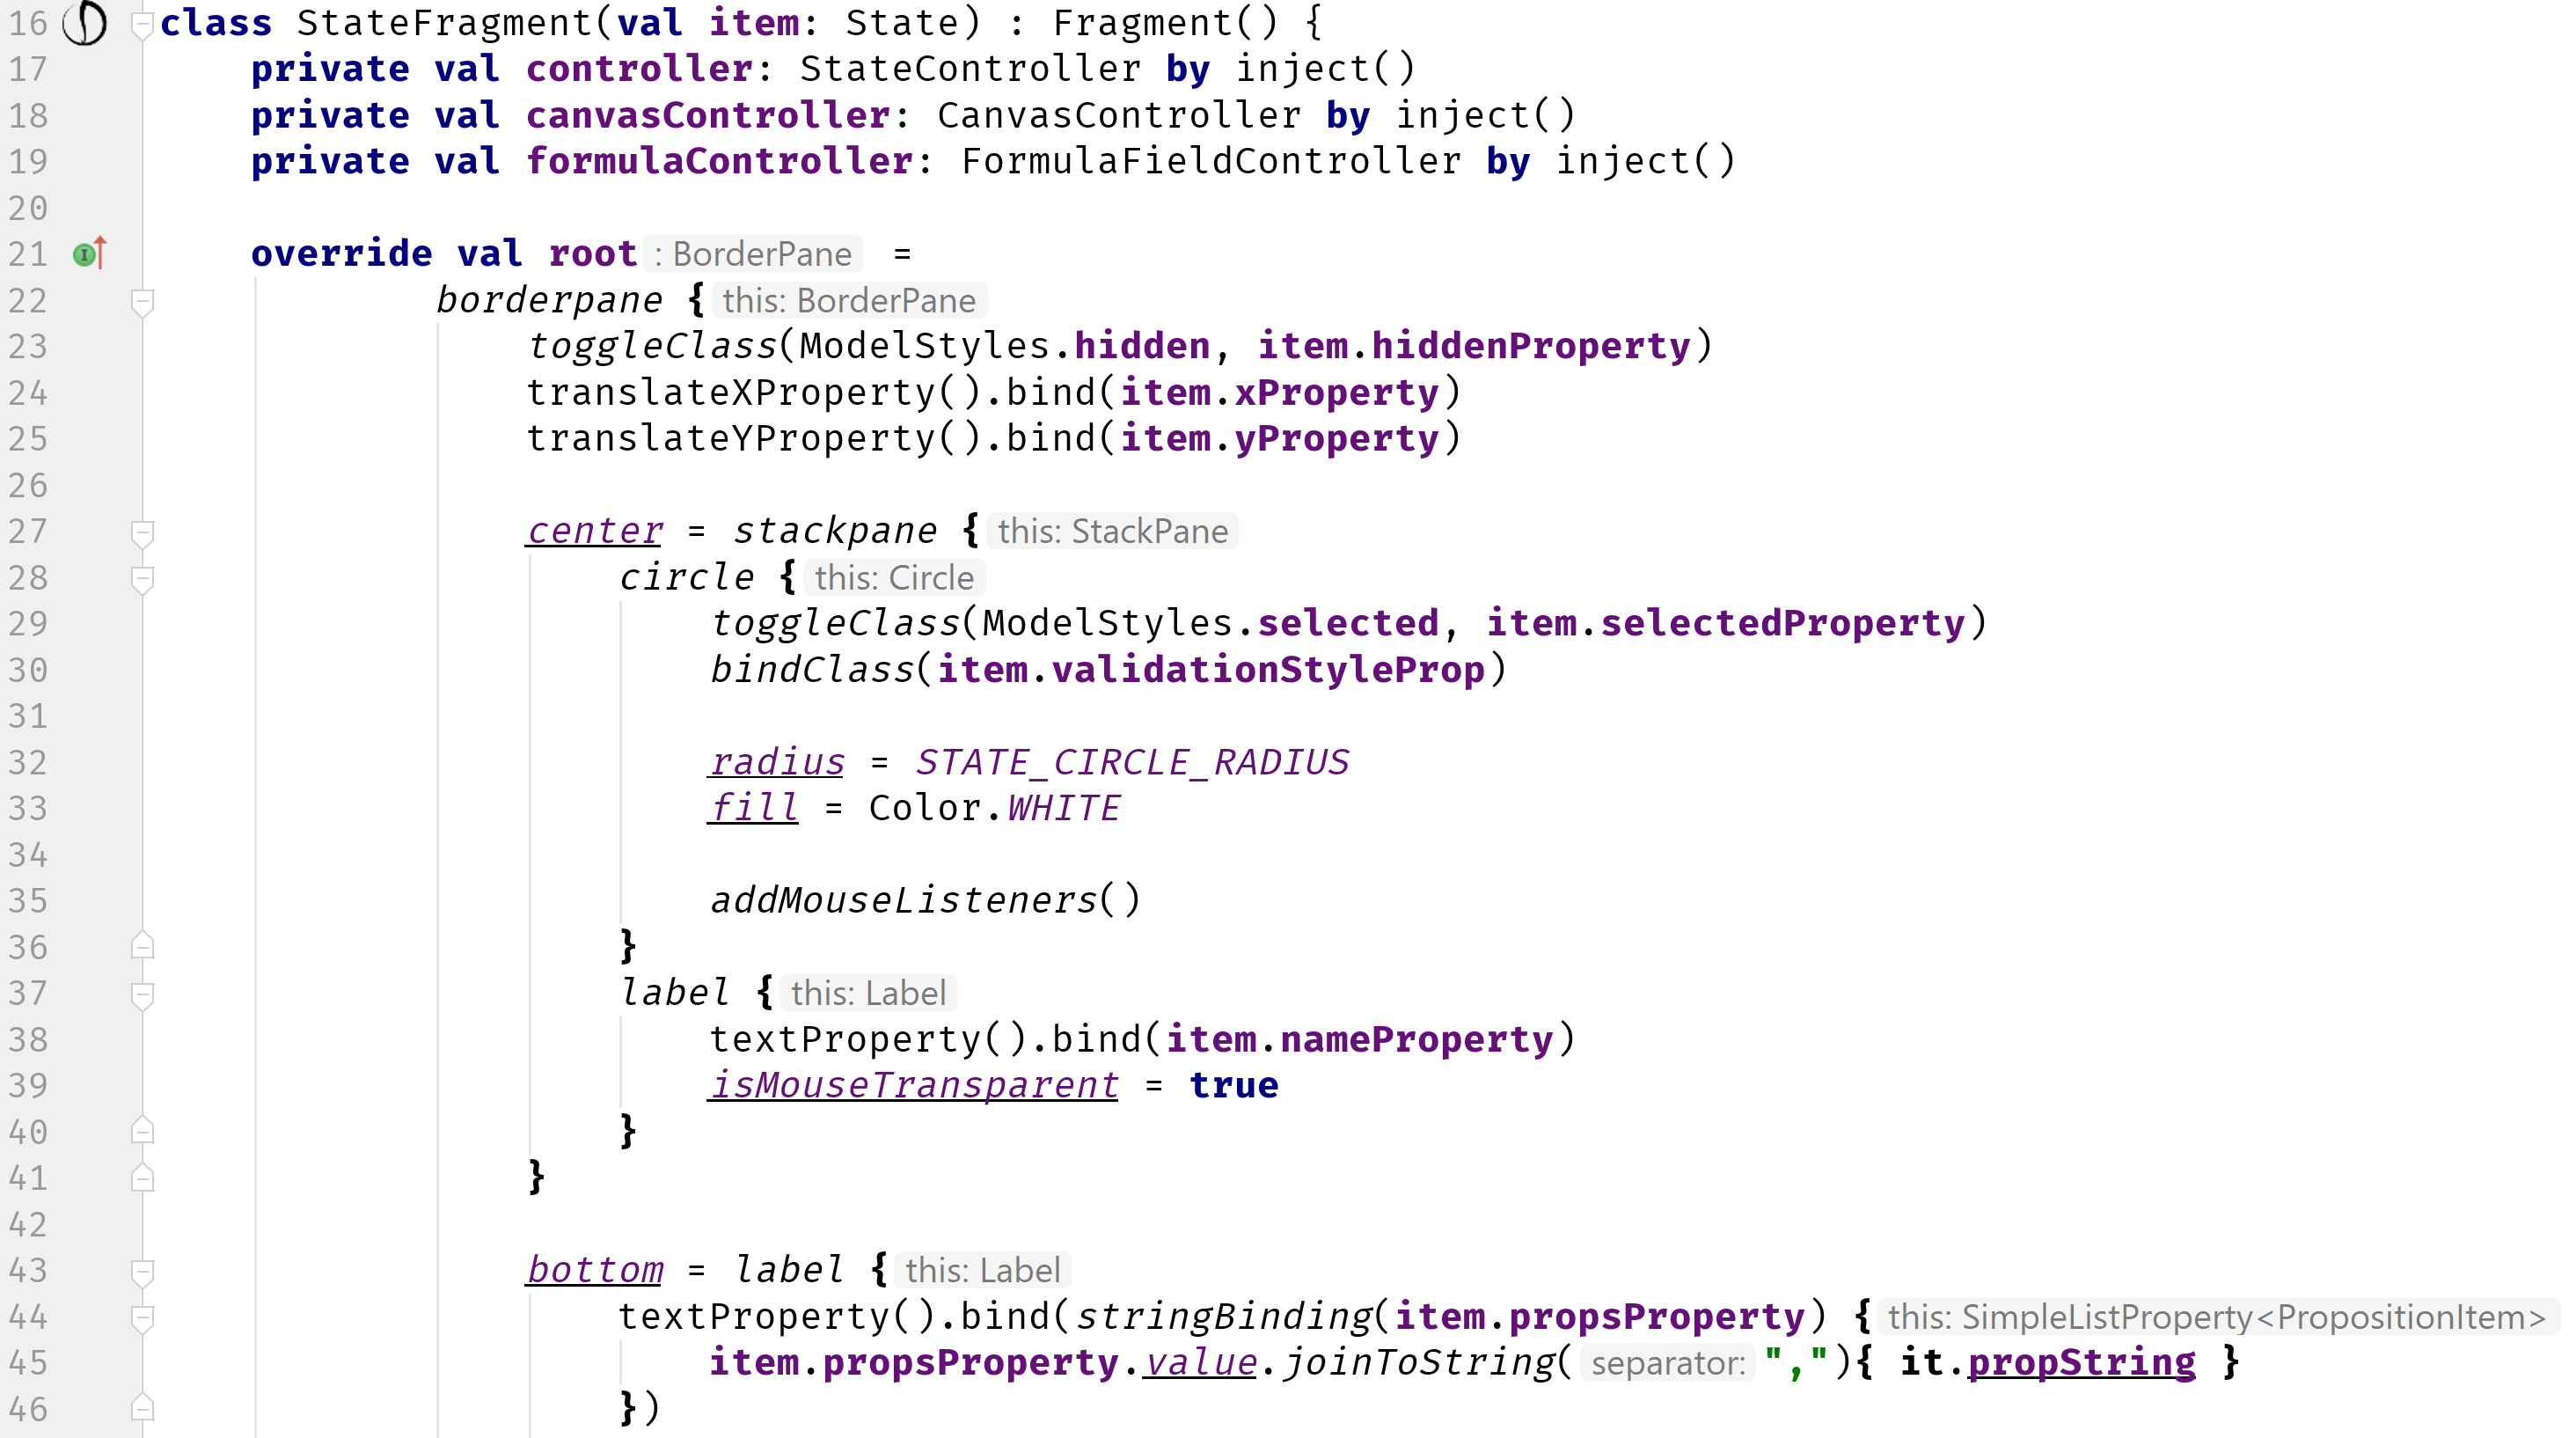
\includegraphics[width=\textwidth]{StateFragmentSnippet.png}
	\caption{Code handling how the UI components representing states are built. Note the conciseness due to implicit contexts.}
	\label{fig:StatFragSnip}
\end{figure}

For these reasons, \cname{} is implemented in Kotlin, as prior to this project, most of my programming experience came from Java and its many libraries and as such, moving to a language with a far more concise syntax but still being able to lean on my previous experience made Kotlin an excellent tool for this complex system. Going back to Java's wealth of libraries, the choice of GUI library to construct our user interface in fell on the \textit{de facto} standard Java GUI library, JavaFX, or more precisely; a Kotlin wrapper for it called TornadoFX \footnote{Library homepage at: \url{https://tornadofx.io}}. The reason for choosing TornadoFX is that while JavaFX is a widely used and mature library with powerful features, its usage also tends to result in clunky and verbose code. JavaFX does admittedly provide a solution to this; dumping most of the layout, styling and positioning of components into specialized XML-files. While this helps clean up classes representing UI-components however, it also makes dynamic component generation clumsier and tends to abstract away the component hierarchy in ways that makes it harder to reason around its structure. TornadoFX on the other hand, being a Kotlin library is able to present a much cleaner API by utilizing Kotlin features such as lambda expressions attached to receivers in order to create composable builder functions which generate your JavaFX component hierarchy in an imperative fashion. Additionally, the wrapper also has excellent and concise shorthands for creating dynamic bindings between UI components and observable sets of data, which we ended up using all throughout the application. However, the primary justification for choosing TornadoFX is how its composable builder functions allow you to circumvent the normally inverse order of declaration and creation of UI components compared to their order in the component hierarchy, which can be seen in Figure \ref{fig:StatFragSnip}.

%Later mention usage of this Java interoperability through JavaFX and Java hook for ANTLR

\subsection{Language and interpretation}

Besides creating an understandable user interface another large challenge we needed to solve was how to convert the plain text the user types in into data structures representing formulas to check. For this, we used a tool called ANTLR (ANother Tool for Language Recognition)\footnote{\url{http://www.antlr.org/}}. ANTLR is a powerful parser generator which based off of a set of grammatical rules, can be used to generate parsers which implement these rules. These grammatical rules can be broadly split into parser and lexer rules. Lexer rules are the low-level rules which define how the tool should convert individual characters or short strings of characters into lexical tokens which are then used by the more high-level parser rules to define how ANTLR should assemble these tokens together again. For a more concrete example, we have the entirety of \cname{}'s grammatical rules pictured in Figure \ref{fig:grammar}. Here we can see how this simple set of lexical rules handle converting symbols into tokens representing the various operators in our language, but also how our set of parser rules define all legal ways of combining these symbols into formulas. 
\begin{figure}[h]
	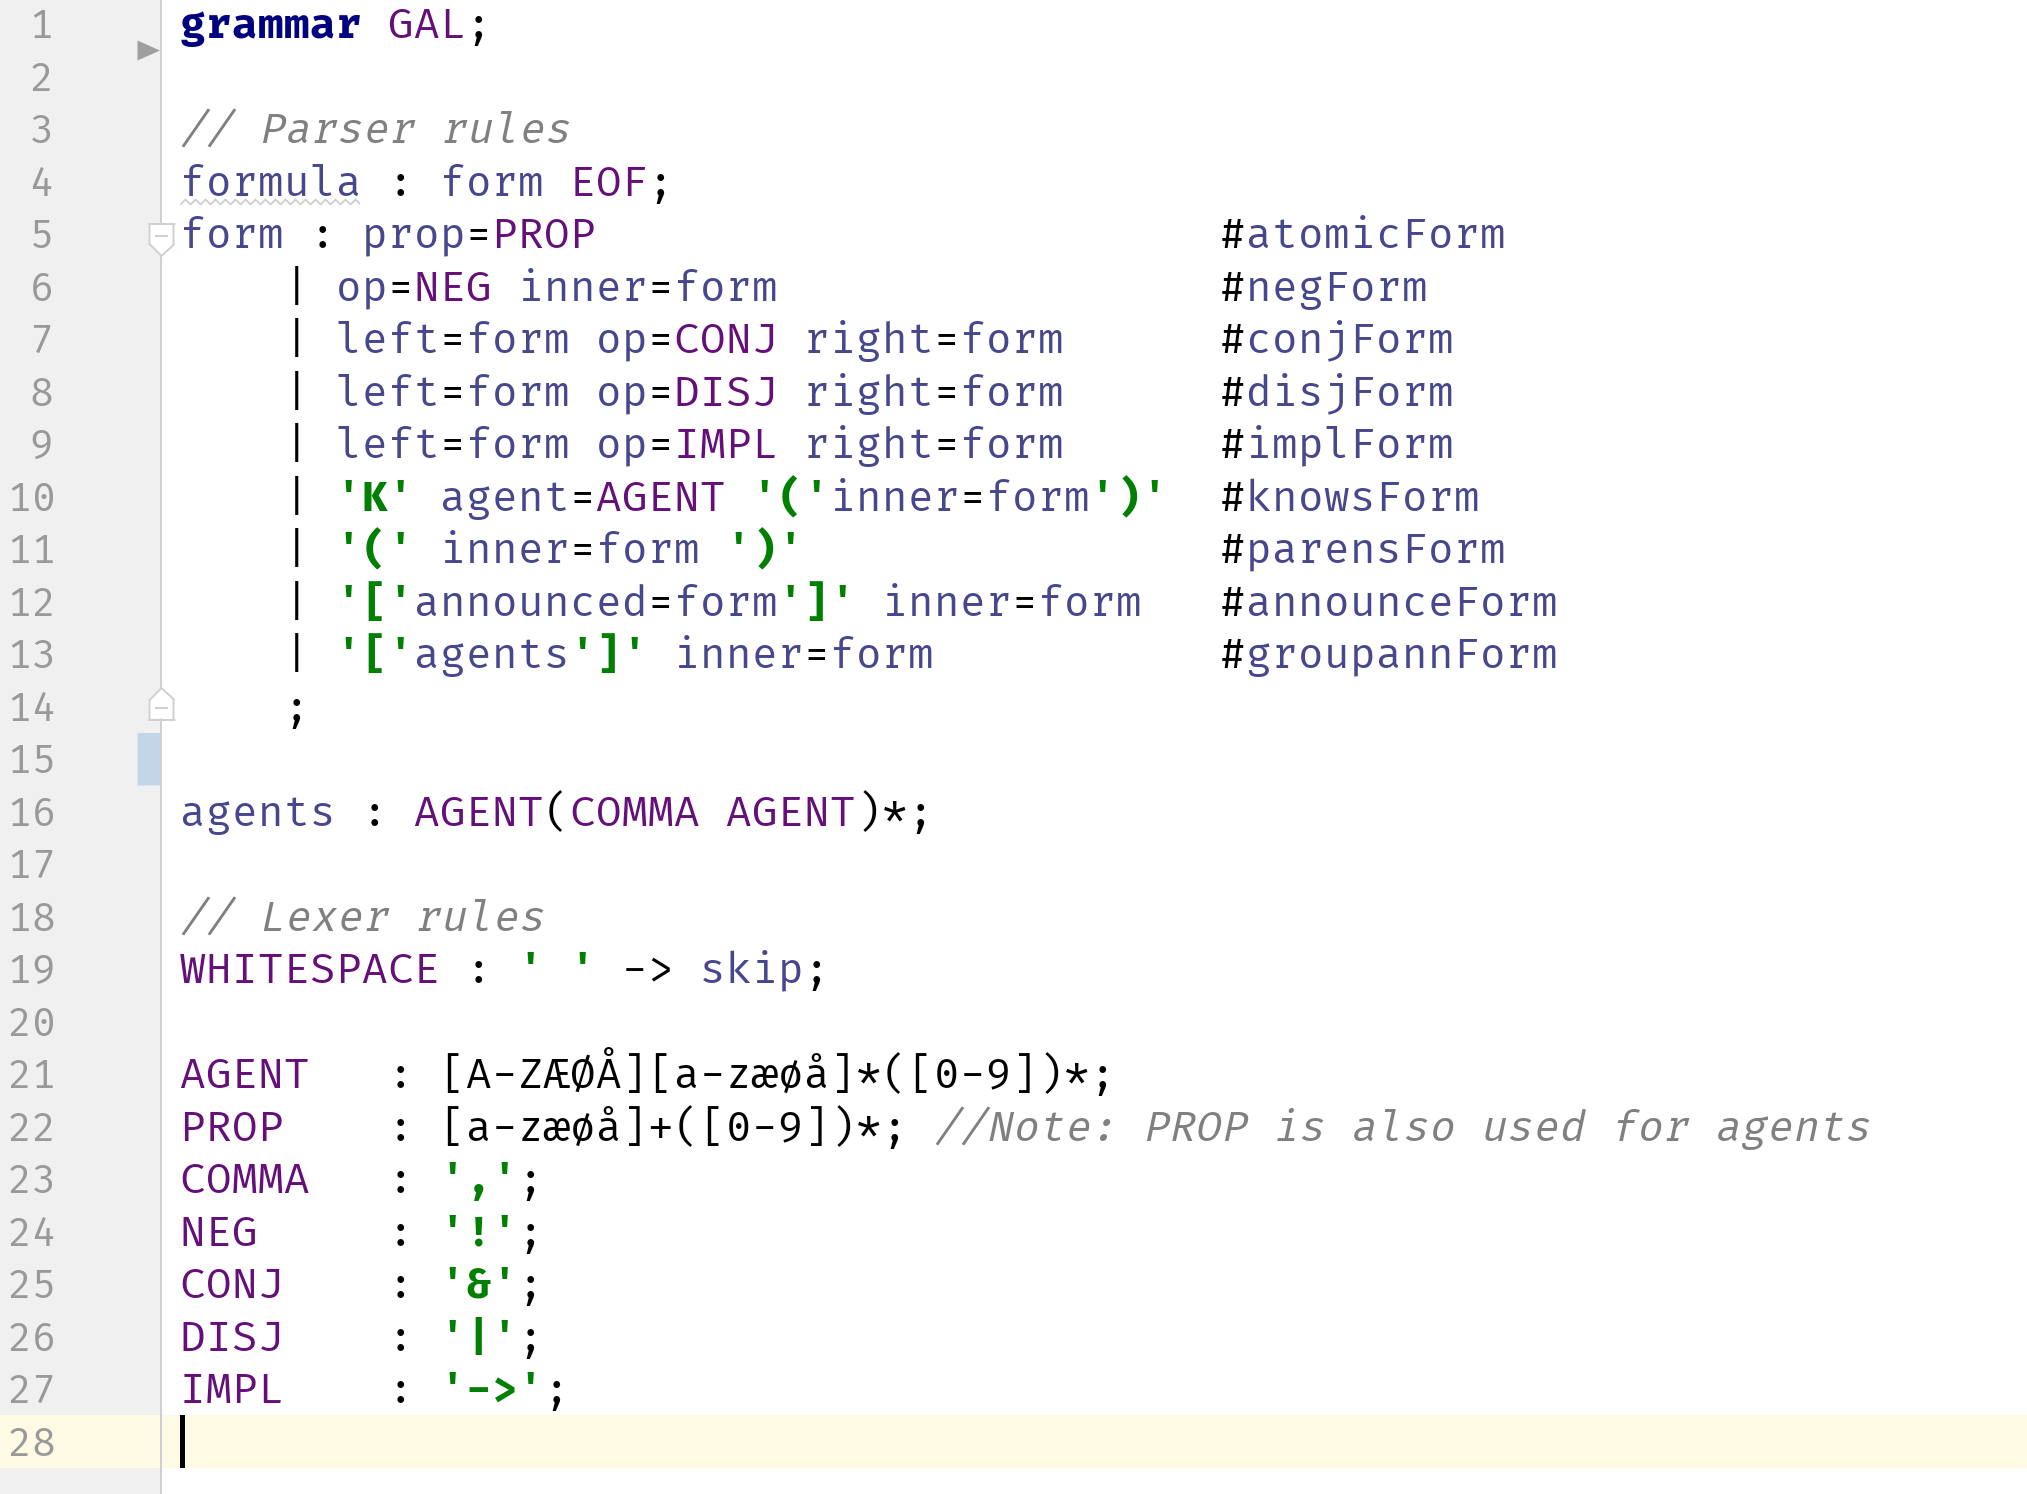
\includegraphics[width = \textwidth]{GALGrammar.png}
	\caption{Grammatical rules for parsing formulas in \cname{} with ANTLR.}
	\label{fig:grammar}
\end{figure}

For comparison, the language described by this ANTLR grammar can also be expressed as the following BNF (terminal symbols are underlined):

\begin{align*}
  \phi ~~&::=~~ \pi ~\big|~ \underline{!} \, \phi ~\big|~ \phi \, \underline{\&} \, \phi ~\big|~ \phi \,\underline{ | }\, \phi ~\big|~ \phi \, \underline{\text{-}\!>} \, \phi ~\big|~ \underline{K}\, \alpha\, \underline{(}\,\phi\,\underline{)} ~\big|~ \underline{(}\, \phi \,\underline{)} ~\big|~ \underline{[} \, \phi \, \underline{]} \, \phi ~\big|~ \underline{[} \, C \, \underline{]}\, \phi\\
  C ~~&::=~~ \alpha ~\big|~ \alpha \, \underline{,}\, C
\end{align*}

where $\pi$ (propositions) and $\alpha$ (agents) are sets of terminal symbols characterized as follows:
$\pi$ contains all strings of at least one lower case letter and possibly followed by a string of digits, matching the following regular expression:
$$
[\text{a-zæøå}]^+[0-9]^*
$$
$\alpha$ is a single upper case letter followed by a (possibly empty) string of lower case letters, and subsequently a (possibly empty) string of digits, as described by the following regular expression:
$$
[\text{A-ZÆØÅ}][\text{a-zæøå}]^*[0-9]^*
$$

One thing to note in Figure \ref{fig:grammar} are the symbols used to represent negation, conjunction and disjunction. As previously mentioned, since the commonly used symbols for these operators do not exist on normal keyboards, the UI would either need extra buttons to facilitate inserting these symbols or use more easily accessible surrogate symbols. Another small concession I had to make in order to differentiate between agents and propositions, was to require that agent names be capitalized, as I would otherwise have to resort to using different symbols to differentiate between regular public announcements and group announcements. 

\begin{figure}[h]
	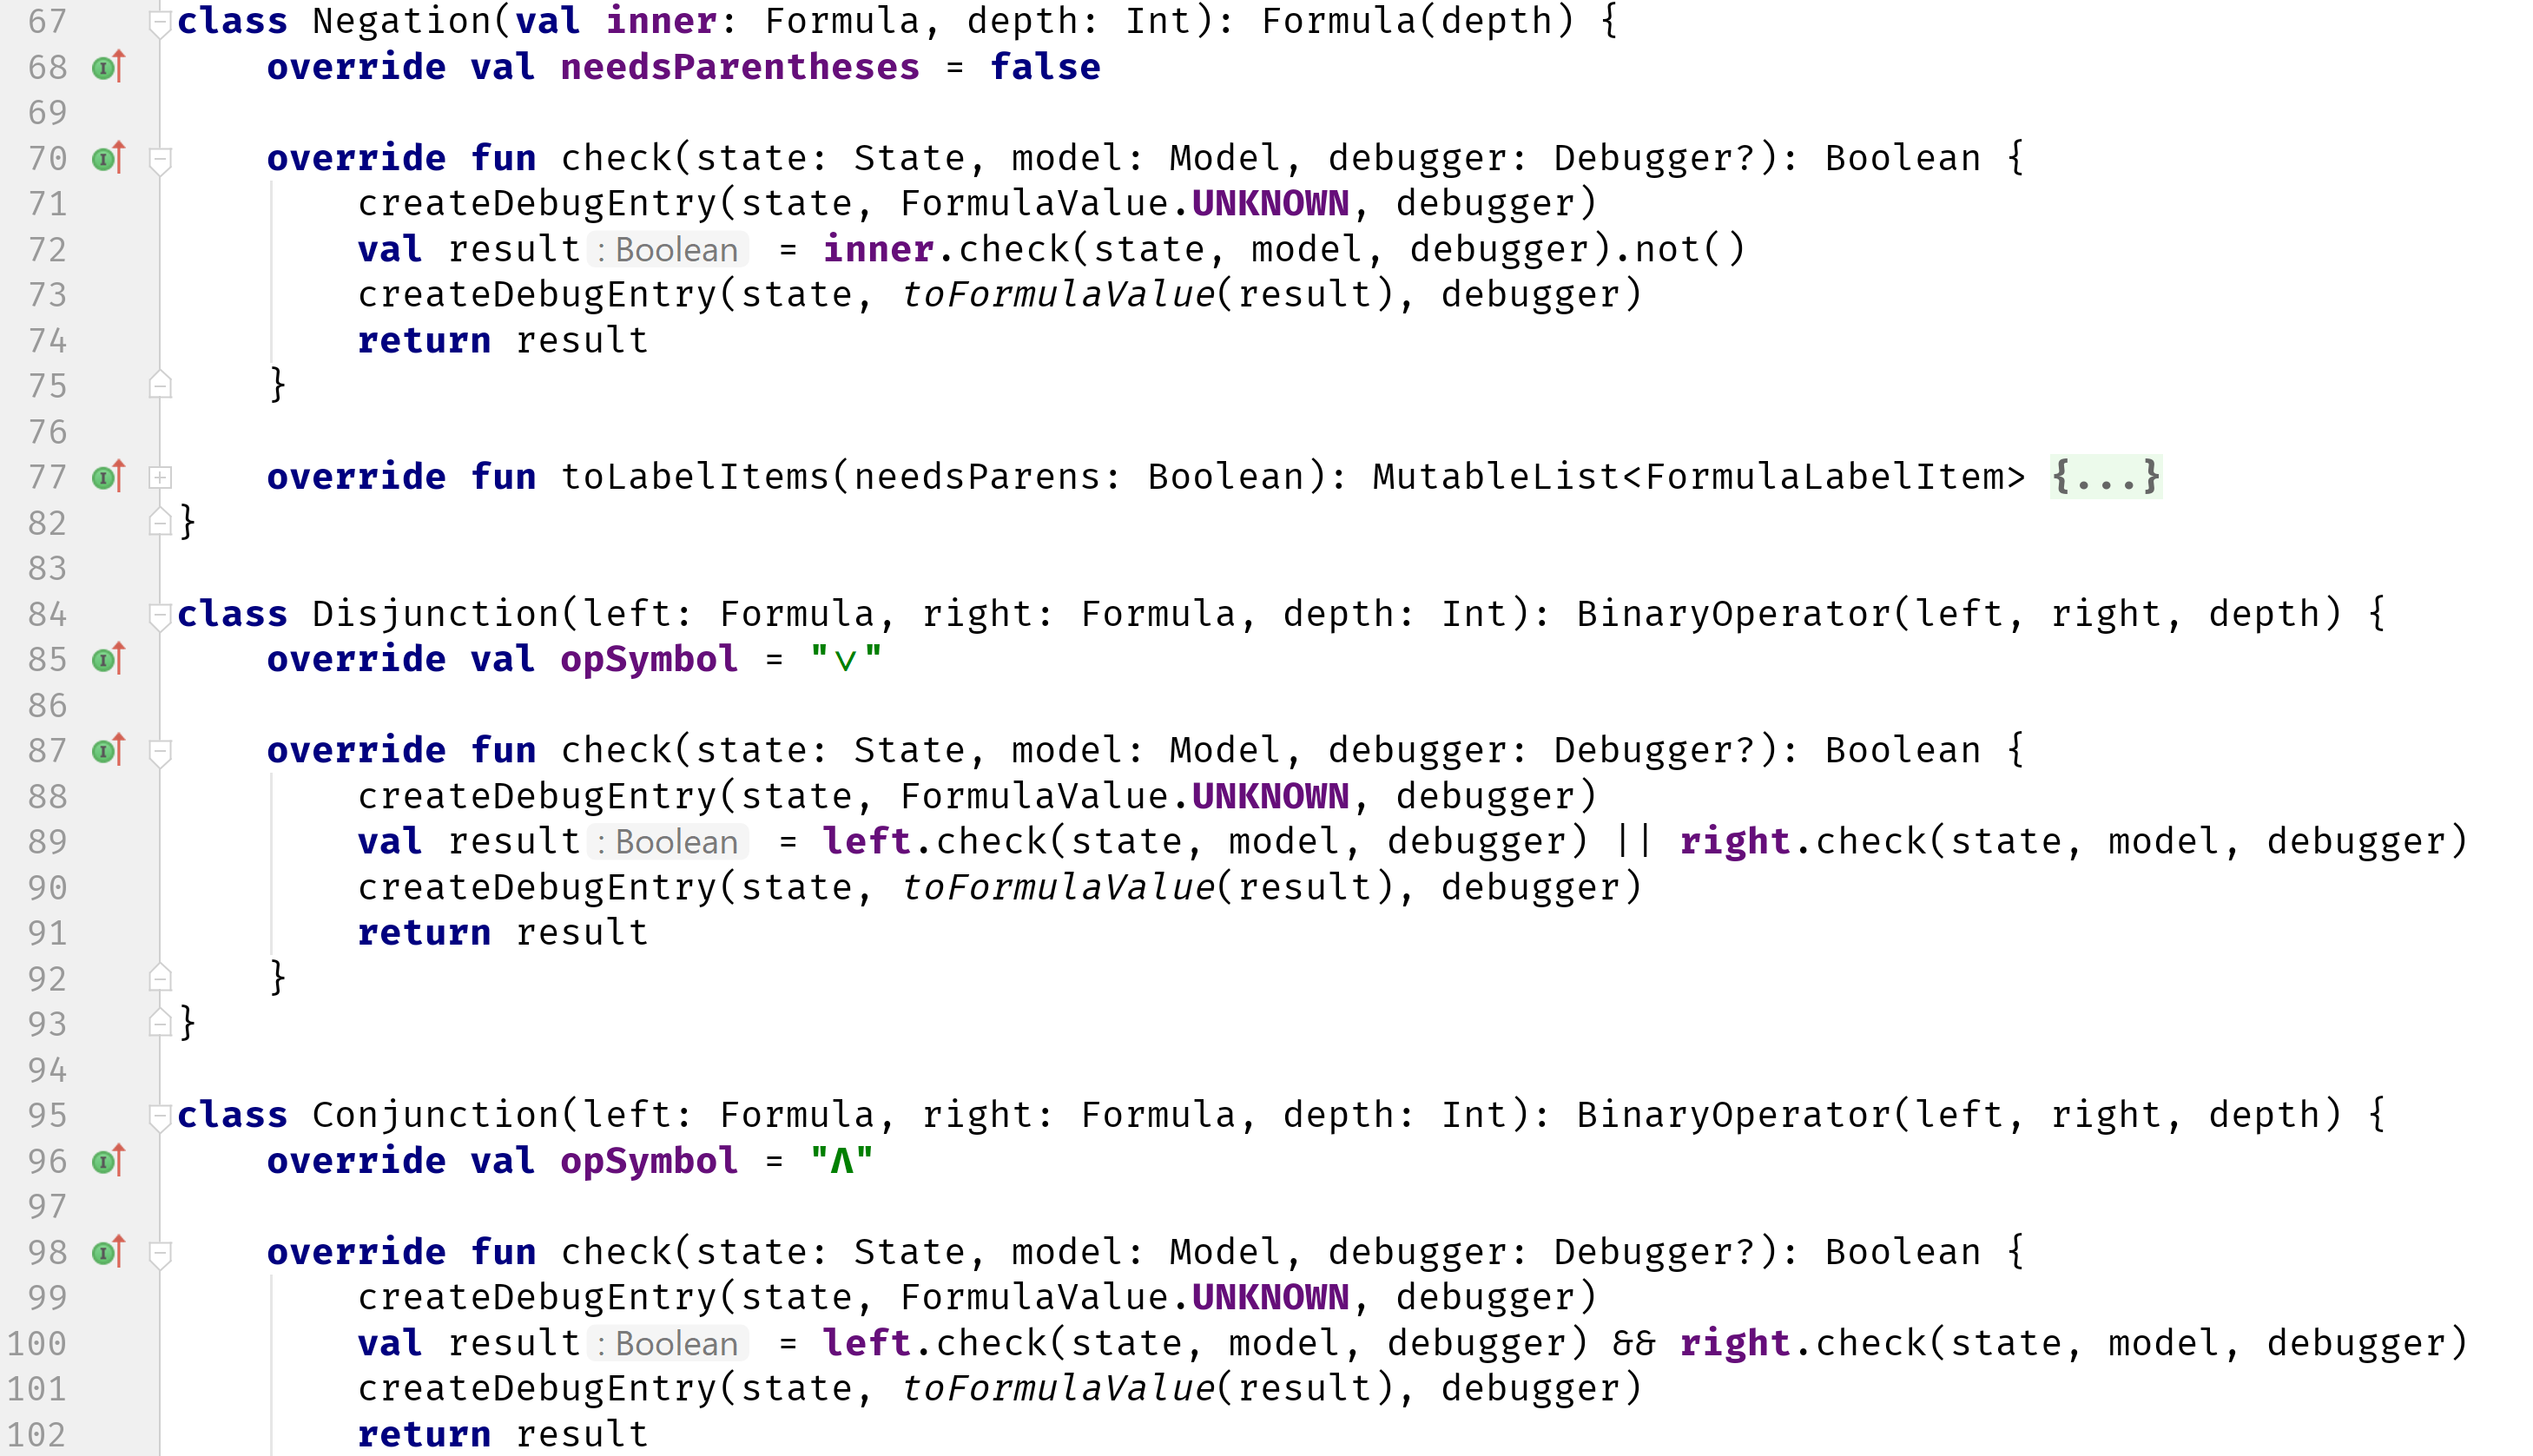
\includegraphics[width=\textwidth]{FormulaImpl.png}
	\caption{Snippet showing how various operators are implemented}
	\label{fig:formulaImpl}
\end{figure}

The parser that ANTLR generates from this simple grammar is then used to convert the user's plain text input into instances of our Kotlin classes which represent the various operators in our language. An interesting thing to note here however is that not only does it create instances of our operators, but it also instantiates them in order of traversal as it builds the formula tree, conserving the structure of this tree as it is rebuilt using our Kotlin-implementations of the operators. One of the more elegant aspects of our design is how these operators were implemented; with each operator extending an abstract formula class and simply overriding it's `check'-function with their own semantics, as can be seen in Figure \ref{fig:formulaImpl}. Also note how the constructors of each operator also takes other formulas as their parameters, allowing us to directly implement the BNF definition of GAL presented earlier through constructor typing alone.

\subsection{Kripke structures and UI components}

As the focus when making the application was mainly on making it as easy to use as possible while presenting information in a visual manner that is easy to grasp, we ended up making several deviations from the more commonly seen logical definitions of epistemic models. In Definition \ref{def:model} we present $\rels$ as a function from each agent to their respective equivalence relation for every state in the model. In \cname{} however, we instead chose to represent these equivalence relations as a set of edges represented as objects consisting of a pair of states and the set of agents that consider this pair of states indistinguishable. The reasons for this ties back into how we wanted to present an interactive view of the models in our application, as TornadoFX, our GUI library makes it far easier to represent each component of our models as concrete objects, which we can then bind UI-components to. Since each edge also has a reference to the set of agents it applies to, this makes it trivial for us to visualize this information as well. 

Building on these changes, we additionally made each state aware of which edges it is connected to, simplifying the process of finding indistinguishable states for a given agent, by enabling us to filter the set of edges our state is connected to based on our given agent and return the list of states these edges lead to. While these are deviations from how Kripke structures are more commonly defined, we argue that they make for a much cleaner programmatic representation as they allowed us to simplify both visualization as well as our implementation of the semantics.

We also chose to flip the valuation function by letting states hold a reference to a set of propositions which are satisfied in them, rather than each proposition being linked to the set of states they are satisfied in. Our reasoning here is much the same as for changing how we handle indistinguishability; it allowed us to simplify how we present which propositions are true in each state. We do so by applying a mapping function to these sets of propositions to generate labels in our UI which can then be automatically updated whenever this underlying set of propositions updates. This is far simpler than having to go through the entire set of propositions each time the user updates which propositions a given state satisfies. The code responsible for binding this set of propositions to labels can be seen at the bottom of Figure \ref{fig:StatFragSnip}.


\subsection{Model checking}

Going back to our presentation of \cname{} in the previous chapter, we described that the tool provides two main modes of checking formulas, which we will now discuss the implementation of. The first and simplest of these modes is simply checking which of the states in the user's model satisfy the input formula. With our implementation of formulas, we can simply do this by invoking the formula's check-function on each state in our model, styling the state-component based on the outcome of this checking, as can be seen in Figure \ref{fig:CheckingFunction}. We also previously described how \cname{} allows its user to mouse over the various subformulas in order to check how they affect the valuation of their containing formula. We implemented this by tying each symbol in the displayed formula to the subformula it represents and then calling the same check-formula with this subformula.

\begin{figure}[h]
	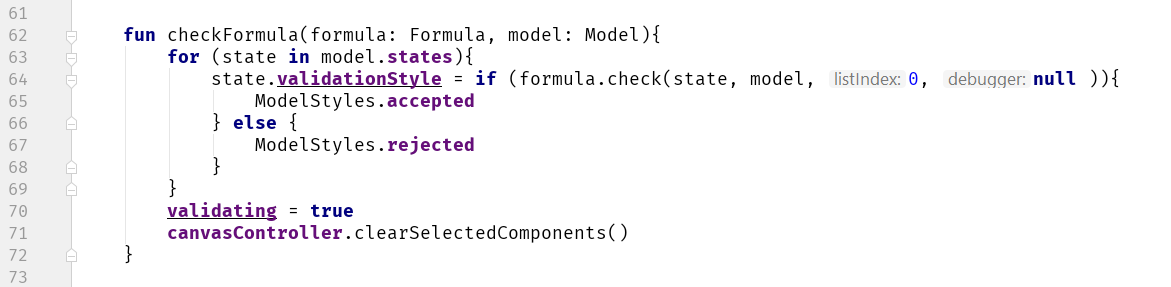
\includegraphics[width=\textwidth]{CheckingFunction.png}
	\caption{Function responsible for highlighting which states in our model satisfy the input formula}
	\label{fig:CheckingFunction}
\end{figure}

How step-by-step visualization works is somewhat more involved. A high-level description of how it is implemented is that the `debugger' hooks into the $check$ function of the formula, and logs each step of the checking process. Looking back at Figure \ref{fig:formulaImpl}, this can be seen through our calls to \textit{createDebugEntry}, which is responsible for logging the valuation of each operator in the user's formula before and after every call to this $check$ function.

Each log then carries information about what the valuations of each operator was at that point in the process, so that this checking process can be played back and visualized in the form of showing the various operators change color as their valuations become known. 

Briefly touching upon saving and loading of models as mentioned at the end of the last chapter, as our models are plain Kotlin (and by extension Java, as Kotlin is fully interoperable with Java) objects, reading and writing them to files is simply a matter of using the built-in tools in the Java library to serialize them and write them to file, as seen in Figure \ref{fig:serialization}. While using the JVM library for writing and reading models from files saved us a lot of time, it does however also mean that the models are written in a plain binary format. While it would have been nice to store our models in a more widely-used format so that more complex models could be visualized and edited in more powerful graph editing tools such as Gephi\footnote{https://gephi.org/}, this was left as future work since I estimated it would take too long to implement compared to the value it would provide.

\begin{figure}
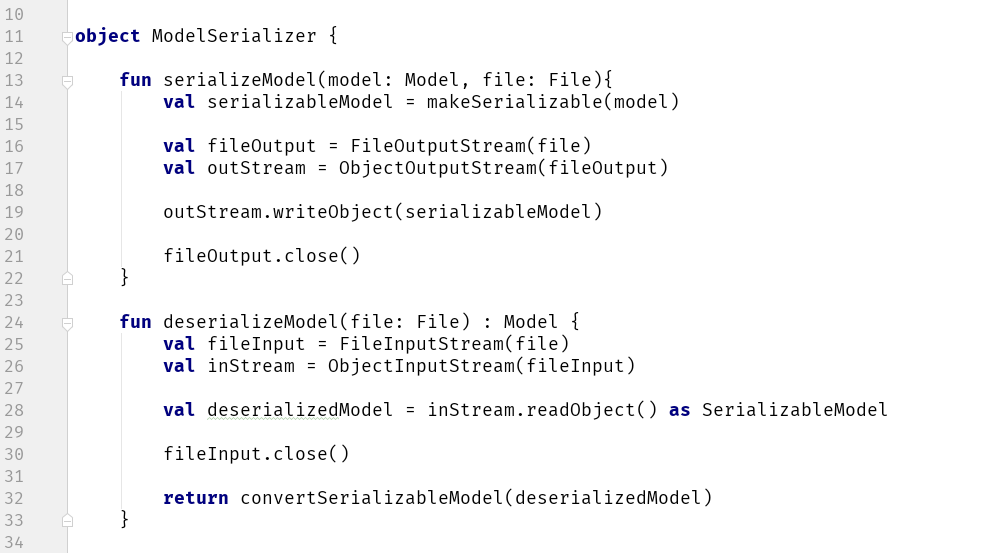
\includegraphics[width=\textwidth]{SerializationCode.png}
\caption{Code behind reading and writing models to file}
\label{fig:serialization}
\end{figure}

%Features - should explain how each of these are implemented \\\\


%Saving and loading models, as well as importing other models into the current model (Useful for importing commonly used components)\\


%Compare with implementations in DEMO, advantages/disadvantages of wrapping things in objects ect.\\
%We use observable objects with pointers to each other, DEMO simply has arrays of integers, which are more lightweight and potentially easier to manipulate, but much harder to render \\
%Discuss differences with logical definitions\\
%Provide walkthrough of how program checks formulas\\

%Debugger, DebugLabels, attaching itself to checking process of formulas, lots of shady voodoo to link DebugEntries in sidepanel to DebugLabels next to each state in order to update them as the user navigates through entries\\

%Debugger inserts callback into CanvasController to know when the user selects a state\\
%List of checking steps has onChange() callback telling the Debugger to apply the valuation map for that step to all formula labels\\

%Checking: Everything up to knowledge is roughly equivalent to logical definitions, minus flipped valuation function. Knowledge is similar, but instead of having an equivalence relation for each agent, each state is instead connected to other states through a set of edges which hold for a set of agents. If 


%Checking, recursive, 'logger' used to display process step-by-step\\

 \newpage
\section{Conclusion}\label{sec:impl}

\subsection{Future work}

%There were also plans for separately visualizing the set of announcements a coalition can make as well as showing what the updated models would look like, but unfortunately this had to be scrapped due to time constraints.


%\todo{Skrive om å måle pedagogisk verdi, muligens peke ut som fremtidlig masteroppgave}

Having developed what we consider to be a potentially highly useful education tool, the big elephant in the room when discussing future work is actually measuring its educational benefit. As both user testing and educational impact studies go beyond the scope of this thesis, we certainly hope that someone might be willing to take up the torch and prove the value of \cname{} in such settings. While \cname{} is fully functional and usable as an educational aid in its current state, there are also a fair few features that we simply did not have time to implement, a few of which we will discuss.

One of the simpler additions to the tool is implementing the dual, also known as `diamond' version of the announcement operators. As these operators do not add any additional expressiveness or capabilities to the model checker they were never prioritized as they can always be expressed through the negation of the box operators. It would still be nice to have support for these operators directly however, to cut down on formula length and complexity when visualizing larger formulas. As both the ANTLR grammar and related formula components are easily extendable, implementing these operators would be fairly trivial as their underlying semantics are basically already implemented.

There are also a fair few additions to the UI we would have liked to implement, such as separately displaying the set of formula extensions a coalition can announce or provide the user with more informative error messages when attempting to parse syntactically incorrect formulas. Visualizing these formula extensions should also not prove all too challenging as the extensions are already generated when checking formulas. Similarly, the ANTLR parsers provide most of the context necessary to present inform the user of which part of their string caused an error, although more complex reasoning around how to parse ambiguous structures in regards to how to handle missing parentheses and the like might be more challenging. 

There were also plans for generalizing \cname{}'s model serializer in order for to be able to export the models as formats beyond its current basic binary format such as GEXF\footnote{\url{https://gephi.org/gexf/format/}} in order to be able to view these models in other tools such as Gephi\footnote{\url{https://gephi.org/}}. As the intended users of the tool are mainly students attempting to gain a better understanding of the semantics of the operators and structures in group announcement logic however, the feature was eventually scrapped as the models created would likely not be all that interesting to visualize in external tools anyway and the work involved would be fairly substantial for a feature that would probably go unused by most users.  Continuing on model serialization, we would also have liked to be able to store additional information or metadata about each model, such as being able to write notes about interesting properties a model might have or formulas that highlight said properties when checked against these models.  \newpage

\newpage

\begin{appendices}

\section*{Appendix A. List of features}\label{sec:impl}

Conclusion pending \newpage

\end{appendices}

\bibliography{library}


\end{document}	